\documentclass{ecnuthesis}

\ecnuSetup {
  % 参数设置
  % 允许采用两种方式设置选项:
  %   1. style/... = ...
  %   2. style = { ... = ... }
  % 注意事项:
  %   1. 请勿在参数设置中出现空行
  %   2. "=" 两侧的空格将被忽略
  %   3. "/" 两侧的空格不会被忽略
  %   4. 请使用英文逗号 "," 分隔选项
  %
  % info 类用于输入论文信息
  info = {
    title = {讲义},
    % 中文标题
    %
    author = {},
    % 姓名
    %
  },
  % style 类用于简单设置论文格式
  style = {
    footnote  = plain,
    % 脚注编号样式
    % 可用选项:
    %   footnote = plain|circled
    % 说明:
    %   plain     脚注的编号仅为数字
    %   circled   脚注的编号为带圆圈数字 (仅限1-10)
    %   (默认选项为 plain )
    %
    numbering = arabic,
    % 章节编号样式
    % 可用选项:
    %   numbering = arabic|alpha|chinese
    % 说明:
    %   arabic    使用数字进行编号 (即理科要求)
    %   alpha     使用字母进行编号 (即外文要求)
    %   chinese   使用汉字进行编号 (即文科要求)
    %   (默认选项为 arabic )
    %
    fontCJK = mac,
    % 中文字体选择
    % 可用选项:
    %   fontCJK = fandol|windows|mac|default
    % 说明:
    %   fandol    使用 TeX 自带的 fandol 字体
    %   windows   使用 Windows 系统内的字体 (中易)
    %   mac       使用 MacOS 系统内的字体
    %   (默认选项为 fandol )
    %
    bibResource = {./source/thesis-ref.bib},
    % 参考文献数据源
    % 由于使用的是 biber + biblatex , 所以必须明确给出 .bib 后缀名
    %
    logoResource = {./source/inner-cover(contains_font).eps},
    % 封面插图数据源
    % 模版已自带, 位于 ./source/inner-cover(contains_font).eps
    % 默认值为空
  }
}

% 需要的宏包可以自行调用
\usepackage{mwe}
\usepackage{graphicx}
\usepackage{float}
\usepackage{subfig}
\usepackage{pifont}
\newcommand\px{\mathrel{/\mkern-5mu/}}  %平行
\newcommand\pxeq{\mathrel{\vcenter{     %平行且等于
\ialign{\hfil##\hfil\crcr
$\scriptstyle\px\!$\crcr
\noalign{\nointerlineskip\vskip1pt}$=$\crcr}}}}
\newcommand\backcong{\mathrel{\reflectbox{$\cong$}}}
\begin{document}

% 设置前置部分编号
\frontmatter

% 中文摘要环境


% 设置正文编号
\mainmatter

\chapter{二次根式}
\chapter{全等三角形}
\chapter{反比例函数}
\section{反比例函数与一次函数}
\section{反比例函数与四边形}
\chapter{一次函数}
\section{斜率与截距}
\begin{definition}
    形如$y=kx+b(k\ne 0)$的函数为一次函数。\\
    $b=0$时为正比例函数,正比例函数也是一次函数。
\end{definition}
\begin{knowledge}
    直线与$x$轴交点为$(-\frac{b}{k},0)$,与$y$轴交点为$(0,b)$
\end{knowledge}
\begin{knowledge}
    $k=\tan \alpha,\alpha$为直线与$x$轴正半轴的夹角。
\end{knowledge}
\begin{knowledge}
    $k=\frac{y_1-y_2}{x_1-x_2}$,$(x_1,y_1),(x_2,y_2)$为直线上两个不同的点。
\end{knowledge}
\begin{knowledge}
    $|k|$越大,直线越陡峭,越接近$y$轴;$|k|$越小,直线越平缓,越接近$x$轴。
\end{knowledge}
\begin{knowledge}
    $k>0$,$y$随着$x$增大而增大;$k<0$,$y$随着$x$增大而减小。
\end{knowledge}
\begin{knowledge}
    若$x$取值范围为$x_1<x<x_2$ \\
    $k>0$时,$f(x_1)$为最小值,$f(x_2)$为最大值。 \\
    $k<0$时,$f(x_1)$为最大值,$f(x_2)$为最小值。
\end{knowledge}
\begin{corollary}
    $k=1$时,直线与$x$轴正半轴夹角为$45^\circ$ \\
    $k=-1$时,直线与$x$轴正半轴夹角为$135^\circ$ \\
    $k=\frac{\sqrt3}{3}$时,直线与$x$轴正半轴夹角为$30^\circ$ \\
    $k=-\frac{\sqrt3}{3}$时,直线与$x$轴正半轴夹角为$150^\circ$ \\
    $k=\sqrt3$时,直线与$x$轴正半轴夹角为$60^\circ$ \\
    $k=-\sqrt3$时,直线与$x$轴正半轴夹角为$120^\circ$
\end{corollary}
\begin{corollary}
    $k=0\Leftrightarrow$直线垂直于$y$轴。$k\to \infty$ 不存在$\Leftrightarrow$直线垂直于$x$轴。
\end{corollary}
\begin{table}[ht]
\centering
\caption{一次函数过的象限}
\begin{tabular}{l|l|l}
 & $b>0$ & $b<0$ \\
\hline
$k>0$ & 一三二 & 一三四 \\
\hline
$k<0$ & 二四一 & 二四三 \\
\hline
\end{tabular}
\end{table}
\begin{problem}
    一次函数$y=kx+b$在定义域$0\le x \le 2$内的最大值为$4$,最小值为$−2$,求一次函数的解析式。
\end{problem}
\begin{problem}
    直线$y=kx+b$不经过第二象限,求$k$和$b$的取值范围。
\end{problem}
\clearpage
\section{平移与对称}
\begin{conclusion}
    将一次函数$y=kx+b$沿着某个方向平移$a(a>0)$个单位。 \\
    向上平移后的解析式为$y=kx+b+a$ \\
    向下平移后的解析式为$y=kx+b-a$ \\
    向左平移后的解析式为$y=k(x+\frac{b}{k}+a)$,即$y=kx+b+ak$ \\
    向右平移后的解析式为$y=k(x+\frac{b}{k}-a)$,即$y=kx+b-ak$ \\
    口诀:左加右减,上加下减。
\end{conclusion}
\begin{conclusion}
    将一次函数$y=kx+b$沿着某个方向作对称变换。\\
    沿着$x$轴对称后的解析式为$y=-kx-b$ \\
    沿着$y$轴对称后的解析式为$y=-kx+b$ \\
    关于原点对称后的解析式为$y=kx-b$
\end{conclusion}
\begin{problem}
    点$C$为直线$y=x$上与原点不重合的点,直线$y=2x+1$与$x$轴和$y$轴分别交于$A,B$两点,
    将直线沿着射线$OC$方向平移$3\sqrt2$个单位,求平移后直线的解析式。\\
    \\
\end{problem}
\begin{problem}
    将一次函数$y=-3x+4$向下平移$1$个单位相当于向\underline{\quad}(填左或右)平移\underline{\quad}个单位。
\end{problem}
\clearpage

\section{垂直直线的斜率关系}
\begin{conclusion}
    若直线$y=k_1x+b_1$与直线$y=k_2x+b_2$相垂直,则有$k_1·k_2=-1$
\end{conclusion}
\begin{example}
    已知坐标系内两点$A(x_1,y_1),B(x_2,y_2)$,求线段$AB$垂直平分线的解析式。\\
    设线段$AB$垂直平分线的解析式为$y=kx+b$,则有: \\
    $\begin{cases}k·\frac{y_1-y_2}{x_1-x_2}=-1 \\ \frac{y_1+y_2}{2}=k·\frac{x_1+x_2}{2}+b \\ \end{cases}$
\end{example}
\begin{corollary}
    \quad \\
    点$(a,b)$关于直线$y=x$的对称点为$(b,a)$ \\
    点$(a,b)$关于直线$y=-x$的对称点为$(-b,-a)$
\end{corollary}
\begin{problem}
    在平面直角坐标系中,定义点$(-b,-a)$为点$(a,b)$的关联点。若一个点和它的关联点在同一个象限,判断该点所在的象限。
\end{problem}
\begin{problem}
    在平面直角坐标系中,$A(0,3),B(4,0)$,点$C$在坐标轴上且满足$CA=CB$,求$C$点坐标。 \\
    \\
\end{problem}
\begin{problem}
    若直线$y_1=3x+2$与直线$y_2=kx+b$关于直线$y=x$对称,求直线$y_2$的解析式。 \\
    \\
\end{problem}

\clearpage
\section{直线交点与方程解的关系}
\begin{knowledge}
    已知直线$y=k_1x+b_1$和直线$y=k_2x+b_2$ \\
    若$k_1\ne k_2$,两条直线有唯一交点。 \\
    若$k_1 = k_2, b_1 \ne b_2$,两条直线平行,没有交点。 \\
    若$k_1 = k_2, b_1 = b_2$,两条直线重合,有无数个交点。
\end{knowledge}
\begin{knowledge}
    直线$y=k_1x+b_1$与直线$y=k_2x+b_2$的交点$(x_0,y_0)$是方程组 \\
    $\begin{cases} k_1x-y+b_1=0  \\ k_2x-y+b_2=0  \\ \end{cases}$的解。\\
    两条直线有唯一交点 $\Leftrightarrow$ 方程组有唯一解。 \\
    两条直线平行 $\Leftrightarrow$ 方程组无解。 \\
    两条直线重合 $\Leftrightarrow$ 方程组有无数解。
\end{knowledge}
\begin{problem}
    设$b>a$,在同一直角坐标系下画出一次函数$y=bx+a$和一次函数$y=ax+b$的图像。\\
\end{problem}
\begin{problem}
    直线$y=3x-1$与直线$y=x-k$的交点在第四象限,求$k$的取值范围。\\
\end{problem}
\clearpage
\section{一次函数与不等式}
\begin{knowledge}
    若一次函数$y=kx+b$与$x$轴交点为$(x_0,0)$,则有: \\
    方程$kx+b=0$的解为$x=x_0$ \\
    若$k>0$,不等式$kx+b>0$的解集为$x>x_0$,不等式$kx+b<0$的解集为$x<x_0$ \\
    若$k<0$,不等式$kx+b>0$的解集为$x<x_0$,不等式$kx+b<0$的解集为$x>x_0$
\end{knowledge}
\begin{knowledge}
    若一次函数$y=k_1x+b_1$与一次函数$y=k_2x+b_2$相交于$(x_0,y_0)$,且$k_1>k_2$,则有: \\
    $k_1x+b_1>k_2x+b_2$的解集为$x>x_0$ \\
    $k_1x+b_1<k_2x+b_2$的解集为$x<x_0$
\end{knowledge}
\begin{knowledge}
    如下图,若一次函数$y=k_1x+b_1$反比例函数$y=\frac{k_2}{x}$两支相交于$N(x_1,y_1),M(x_2,y_2)$两点,则有:\\
    $k_1x+b_1>\frac{k_2}{x} \Leftrightarrow x_1<x<0$或$x>x_2$\\
    $k_1x+b_1<\frac{k_2}{x} \Leftrightarrow x<x_1$或$0<x<x_2$
\end{knowledge}
\begin{figure}[ht]
\centering
\begin{minipage}[t]{0.48\textwidth}
\centering
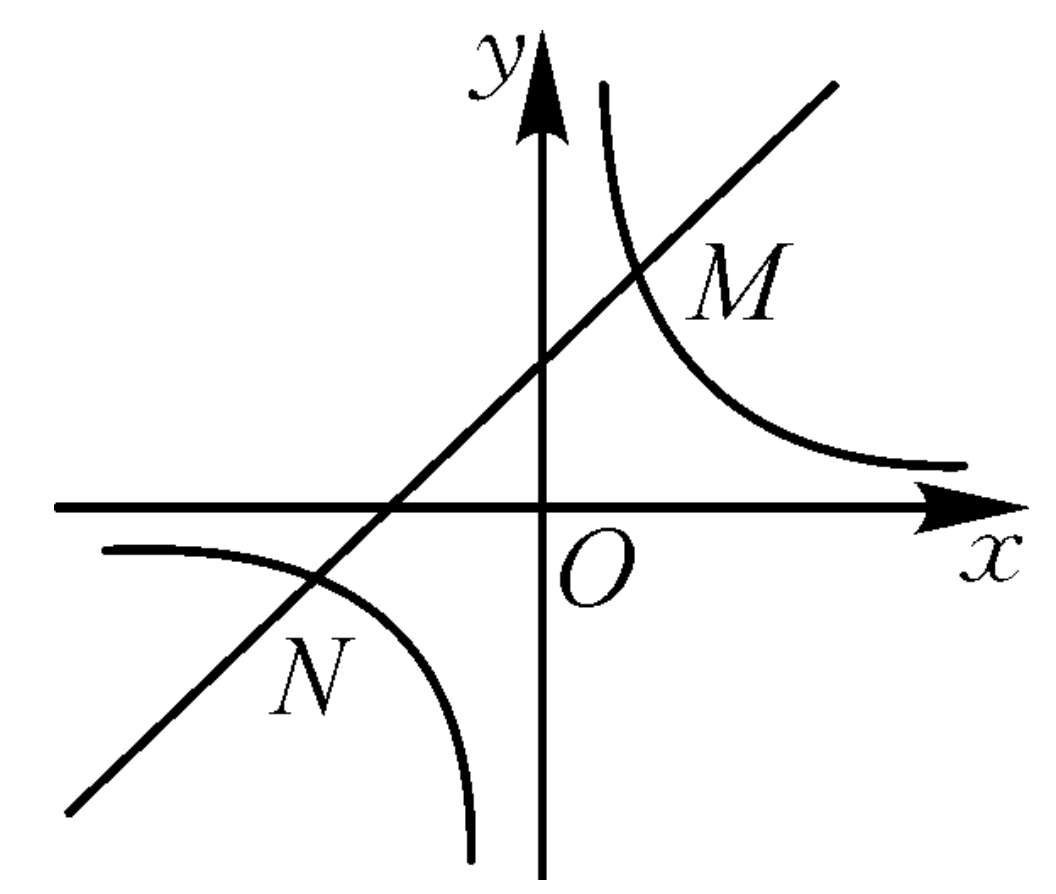
\includegraphics[width=4cm]{picture/4_5_1.png}
\caption{一次函数与反比例函数}
\end{minipage}
\begin{minipage}[t]{0.48\textwidth}
\centering
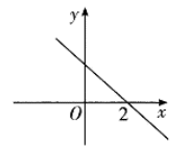
\includegraphics[width=4cm]{picture/4_5_2.png}
\caption{习题4.5.1图}
\end{minipage}
\end{figure}
\begin{problem}
    如图,一次函数$y=kx+b$与$x$轴交于$(2,0)$,求不等式$kx+b>3k$的解集。 \\
\end{problem}
\begin{problem}
    一次函数$y=k_1x+b_1$和一次函数$y_2=k_2x+b_2$满足无论$x$取何值,$y_1>y_2$恒成立,判断$k_1$与$k_2$,$b_1$与$b_2$的关系。\\
\end{problem}
\begin{problem}
    一次函数$y_1=3x+2$和一次函数$y_2=\frac{1}{3}x-\frac{2}{3}$满足$x>m$时,$y_1>y_2$恒成立,求$m$的取值范围。\\
\end{problem}
\begin{problem}
    已知$f(x)=x-1,g(x)=\frac{2}{x}$,定义$h(x)=\max(f(x),g(x))$,
    其中$\max(a,b)=\begin{cases} a & \text{$a \ge b$} \\ b & \text {$a<b$}\end{cases}$,即取两者的最大值。
    求$h(x)$的最小值。
\end{problem}
\clearpage
\section{一次函数中的坐标轴问题}
\begin{problem}
    直线$y=kx+5$与坐标轴围成的三角形的周长为30,求$k$的值。\\
    \\
\end{problem}
\begin{problem}
    直线$y=kx-3$与坐标轴围成的三角形的面积为6,求$k$的值。\\
    \\
\end{problem}
\begin{problem}
    直线$y=kx+b$图像经过点$P(3,2)$且与$x$轴正半轴和$y$轴正半轴分别交于$A,B$两点,且$OA+OB=12$,求一次函数的解析式。\\
    \\
\end{problem}
\clearpage
\section{一次函数中的面积问题}
\begin{knowledge}
    如图,$\triangle ABC$面积可以表示为$\frac{1}{2}$水平宽·铅垂高。\\
    设$A(x_1,y_1),B(x_2,y_2),C(x_3,y_3)$ \\
    根据$A,B$坐标算出直线的解析式,求出$D$点坐标$(x_4,y_4)$ \\
    $S_{\triangle ABC}=\frac{1}{2}|x_2-x_1||y_3-y_4|$ \\
    若$C$点恰好在坐标原点,铅垂高即为一次函数的截距取绝对值。
\end{knowledge}
\begin{figure}[ht]
\centering
\begin{minipage}[t]{0.48\textwidth}
\centering
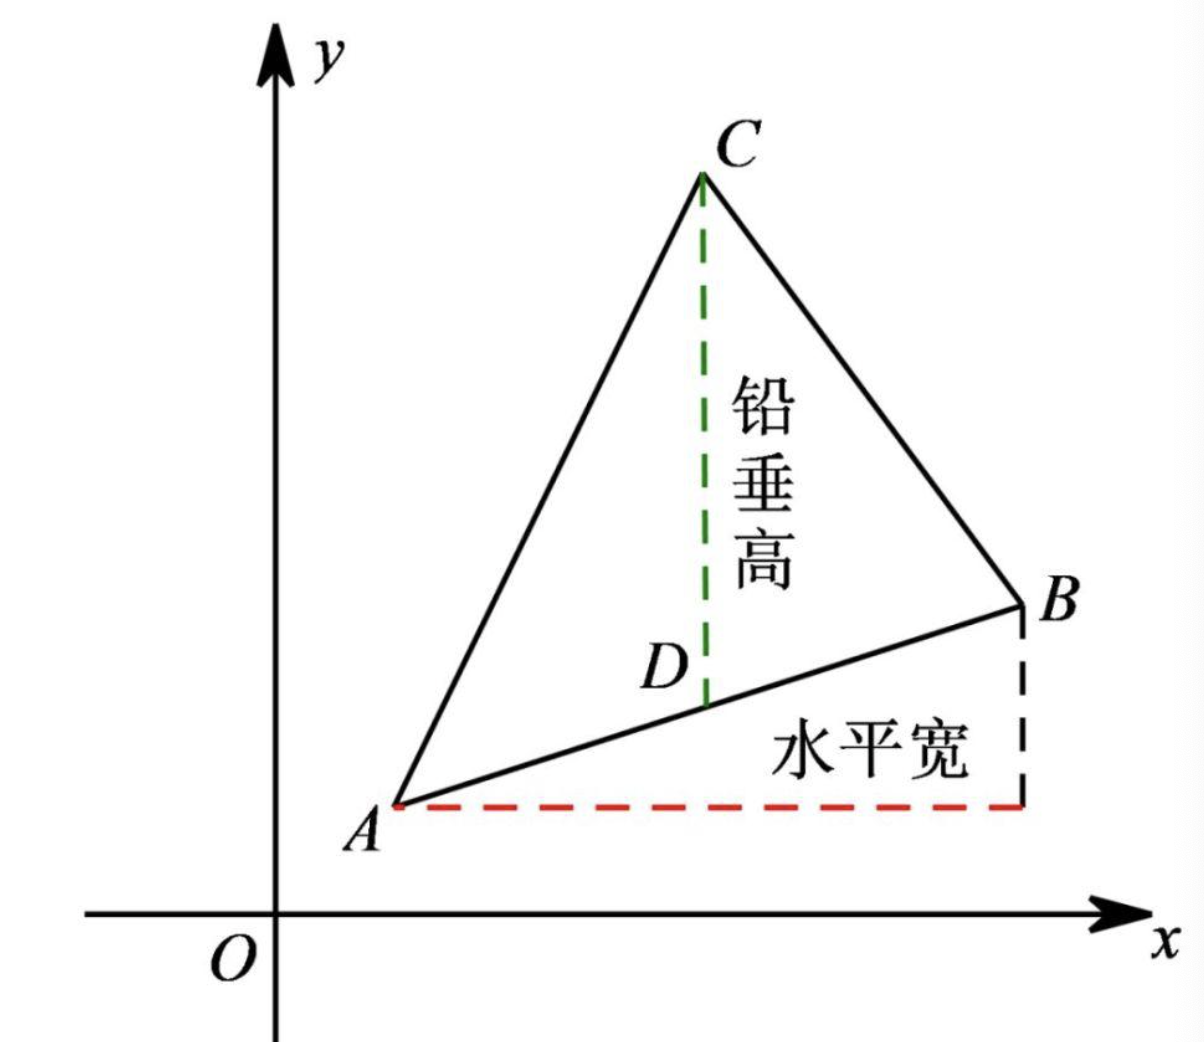
\includegraphics[width=4cm]{picture/4_7_1.png}
\caption{铅垂法}
\end{minipage}
\hfill
\begin{minipage}[t]{0.48\textwidth}
\centering
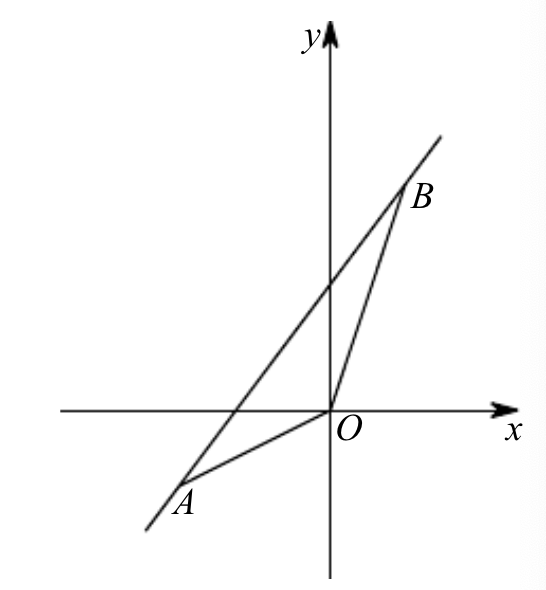
\includegraphics[width=4cm]{picture/4_7_2.png}
\caption{有一个顶点在原点的三角形}
\end{minipage}
\end{figure}
\begin{problem}
    //todo
\end{problem}
\clearpage
\section{一次函数过定点问题}
\begin{example}
    求一次函数$y=(2-k)x+3k$过的定点。 \\
    一次函数过定点,说明存在一组点$(x,y)$满足无论$k$取何值,等式$y=(2-k)x+3k$恒成立。 \\
    说明$k$的所有系数为零。 \\
    $(3-x)k+2x-y=0$ \\
    $\begin{cases} 3-x=0 \\ 2x-y=0 \\ \end{cases} \Rightarrow x=3,y=6$ \\
    所以一次函数过定点(3,6)
\end{example}
\begin{problem}
    若$(2k−1)x−(k−3)y−(k−4)=0$是$y$关于$x$的一次函数,求$k$的取值范围,并求出当$k$满足取值范围时,一次函数恒过的定点。\\
    \\
\end{problem}
\begin{problem}
    平面直角坐标系有两点$A(4,5),B(6,9)$,若一次函数$y=kx−2k+3$与线段$AB$有交点,求$k$的取值范围。\\
    \\
\end{problem}
\clearpage
\section{一次函数与将军饮马问题}
\begin{knowledge}
    如图,在直线$l$上找一点$P$,使得以下结论成立。 \\
    $PB+PA$最小,作$B$关于$l$的对称点$B'$,$P$为$AB'$与$l$的交点。最小值为$AB'$\\
    $|PA-PB|$最小,$P$为线段$AB$垂直平分线与$l$的交点。最小值为0 \\
    $|PA-PB|$最大,$P$为$AB$延长线与$l$的交点。最大值为$AB$ \\
\end{knowledge}
\begin{figure}[ht]
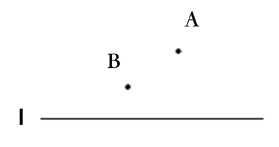
\includegraphics[width=4cm]{picture/4_9_1.png}
\caption{将军饮马}
\end{figure}
\begin{problem}
    已知平面直角坐标系两点$A(2,3),B(4,5)$,$C$在$x$轴上,求满足下列条件的$C$的坐标以及相应的最值。\\
    (1)$CA+CB$最小 \\
    \\
    (2)$|CA-CB|$最小 \\
    \\
    (3)$|CA-CB|$最大 \\
\end{problem}
\begin{problem}
    求根式$\sqrt{x^2-4x+13}+\sqrt{x^2-8x+41}$的最小值,并求出取最小值时$x$的取值。 \\
\end{problem}
\begin{problem}
    求根式$\sqrt{x^2-8x+41}-\sqrt{x^2-4x+13}$的最大值,并求出取最大值时$x$的取值。 \\
\end{problem}
\begin{problem}
    已知平面直角坐标系两点$A(4,6),B(6,4)$,$C$在$y$轴上,$D$在$x$轴上,求使得四边形$ABCD$周长最小的$D$点坐标。\\
\end{problem}

\clearpage
\section{一次函数夹角问题}
\clearpage
\section{一次函数几何综合}
\begin{problem}
    已知一次函数$y=-2x+4$的图像与$x$轴、$y$轴分别交于点$B,A$,以$AB$为边在第一象限内作等腰直角三角形$ABC$,且$\angle ABC=90^\circ$,
    $BA=BC$,作$OB$的垂直平分线$l$交直线$AB$于点$E$,交$x$轴于点$G$. \\
    (1)求点$C$的坐标。
    (2)在$OB$垂直平分线$l$上有一点$M$,且点$M$与点$C$位于直线$AB$的同侧,使得$2S_{\triangle ABM}=S_{\triangle ABC}$,求点$M$的坐标。\\
    (3)在(2)的条件下,联结$CE,CM$, 判断$\triangle CEM$的形状,并给予证明。
\end{problem}
\begin{figure}[H]
\centering
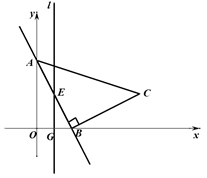
\includegraphics[width=4cm]{picture/401.png}
\caption{练习图}
\end{figure}
\clearpage
\section{一次函数图像分析}
\begin{problem}
    甲、乙两人在笔直的湖边公路上同起点、同终点、同方向匀速步行2400米,先到终点的人原地休息。
    已知甲先出发4分钟,在整个步行过程中,甲、乙两人间的距离(米)与甲出发的时间(分)之间的关系如图中折线
    $OA-AB-BC-CD$所示。\\
    (1)求线段$AB$的表达式,并写出自变量$x$的取值范围。 \\
    (2)求乙的步行速度。 \\
    (3)求点$C,D$的坐标。
\end{problem}
\begin{figure}[H]
\centering
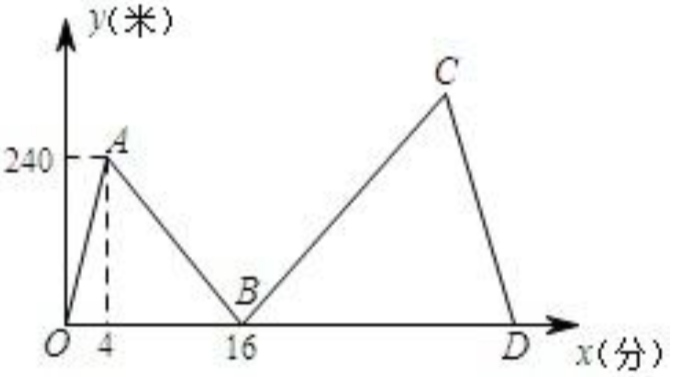
\includegraphics[width=6cm]{picture/6122.png}
\caption{练习图}
\end{figure}
\clearpage
\section{一次函数与实际应用}
\begin{problem}
某自来水公司每月用水收费标准如下:每月固定水处理费$a$元,若当月用水量未超过$b$升,每升水价格为$c$元。
若超过$b$升,超过的部分每升水的单价为$1.5c$元。已知当月有三户人家用水量与计价如下表所示,求$a,b,c$的值。
\end{problem}
\begin{table}[ht]
\centering
\caption{用户用水量}
\begin{tabular}{|l|l|l|}
\hline
用户 & 用水量(升) & 价格(元) \\
\hline
A & 6 & 16 \\
\hline
B & 8 & 20 \\
\hline
C & 16 & 42 \\
\hline
\end{tabular}
\end{table}
\clearpage
\section{点到直线距离公式}
\clearpage
\chapter{代数方程}
\section{一元一次方程与不等式}
\clearpage
\section{一元二次方程与不等式}
\clearpage
\section{分式方程}
\clearpage
\section{无理方程}
\clearpage
\section{根与增根问题}
\begin{knowledge}
    分式方程的增根是去分母后所得整式方程的根,且使得分母为零。\\
    无理方程的增根可能使得根号为负,或者不满足无理方程本身。
\end{knowledge}
\begin{problem}
    分式方程$\frac{6}{(x-1)(x+1)}-\frac{3m}{x-1}-1=0$有增根$x=1$,求$m$的值。\\
\end{problem}
\begin{problem}
    分式方程$\frac{4x}{4-x^2}+1=\frac{k-k^2}{x-2}+\frac{1}{x+2}$不会出现增根,求$k$的取值范围。 \\
\end{problem}
\begin{problem}
    分式方程$\frac{2}{x}-\frac{x-m}{x^2-x}=1+\frac{1}{x-1}$在实数范围内无解,求$m$的值。\\
\end{problem}
\begin{problem}
    无理方程$\sqrt{2x-4}-\sqrt{x+a}=1$有一个增根为4,求$a$的值。\\
\end{problem}
\begin{problem}
    无理方程$\sqrt{4-2x}-kx+2=0$有实数根,求$k$的取值范围。\\
\end{problem}
\begin{problem}
    无理方程$\sqrt{x^2+2x+3}+k=0$有实数根,求$k$的取值范围。\\
\end{problem}
\begin{problem}
    无理方程$\sqrt{x+3}+2x+m=0$只有一个实数根,求$m$的取值范围。\\
\end{problem}
\clearpage
\section{高次方程组的解法}
\clearpage
\section{方程组}
\clearpage
\section{应用}
\begin{problem}
    有一项工程,甲单独做比甲乙合做完工的天数多5天,若甲乙先合做4天,再由乙单独做3天,则能完成全部工程的一半,求甲、乙单独完成此项工程各需几天。
\end{problem}
\clearpage
\chapter{四边形}
\section{多边形}
\begin{conclusion}
    对于$n$边形,有如下结论成立: \\
    内角和为$(n-2)·180^{\circ}$ \\
    外角和为$360^{\circ}$ \\
    最多有3个锐角 \\
    一共有$\frac{n(n-3)}{2}$条对角线 \\
    从一个顶点出发有$n-3$条对角线,将$n$边形分成$n-2$个三角形 \\
\end{conclusion}
\begin{problem}
    $n$边形每增加一条边,会增加多少条对角线? \\
\end{problem}
\begin{problem}
    $m$边形从一个顶点出发沿着对角线将$m$边形分成了7个三角形,$n$边形没有对角线,$k$边形有$k$条对角线,求$(m-k)^n$的值。\\
\end{problem}
\begin{problem}
    如图,正三角形、正方形、正五边形按如图所示位置摆放,求$\angle 1 +\angle 2 + \angle 3$的度数。
\end{problem}
\begin{figure}[H]
\centering
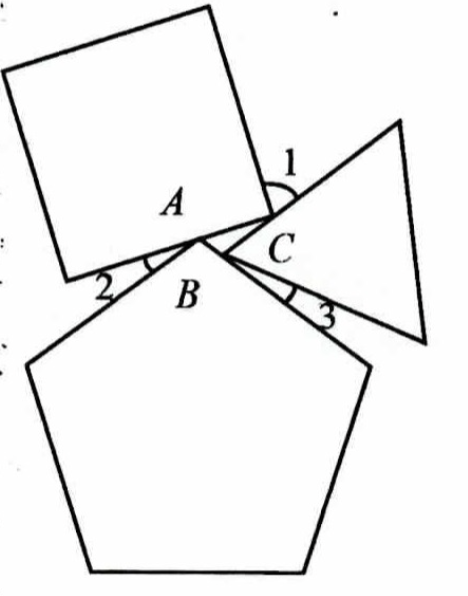
\includegraphics[width=3cm]{picture/6_1_2.png}
\caption{正三角形、正方形与正五边形}
\end{figure}
\begin{problem}
    如图,六边形六个内角都为$120^\circ$,求六边形的周长。
\end{problem}
\begin{figure}[H]
\centering
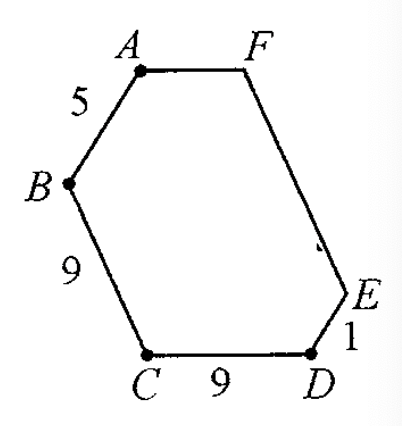
\includegraphics[width=3cm]{picture/647.png}
\caption{六边形}
\end{figure}
\begin{problem}
    定义有三个角相等的四边形为三等角四边形。\\
    (1)在三等角四边形$ABCD$中,$\angle A=\angle B=\angle C$,求$\angle A$的取值范围。 \\
    \\
    (2)如图1,折叠平行四边形$DEBF$使得点$E,F$分别落在边$BE,BF$上的点$A,C$处,折痕为$DG,DH$,求证:四边形$ABCD$为三等角四边形。\\
    \\
    (3)如图2,三等角四边形$ABCD$中,$\angle A=\angle B=\angle C$,$AB=5,AD=\sqrt{26},DC=7$,求$BC$的长度。 \\
    \\
\end{problem}
\begin{figure}[H]
\centering
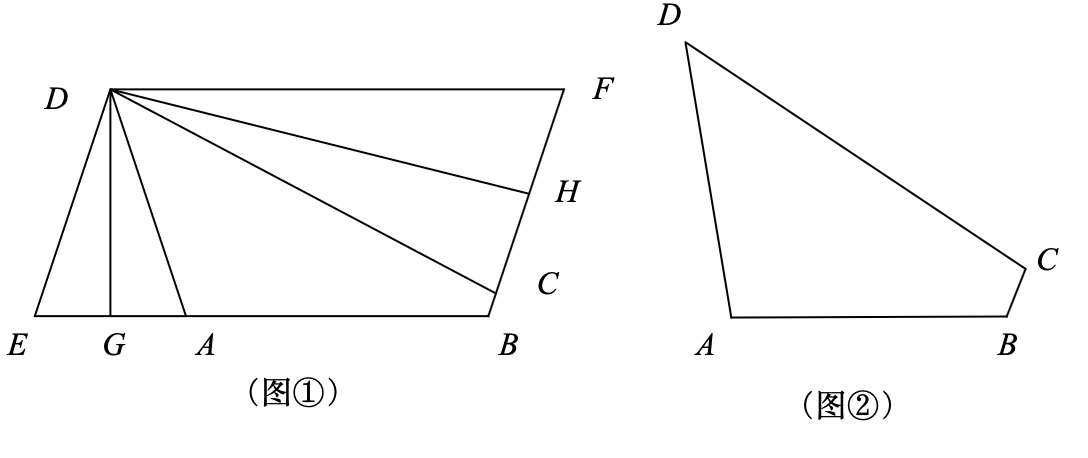
\includegraphics[width=8cm]{picture/6_1_1.png}
\caption{三等角四边形}
\end{figure}
\begin{problem}
    定义至少有一组对边相等的四边形叫等对边四边形。\\
    (1)如图,在$\triangle ABC$中,点$D,E$分别在$AB,AC$上,$CD,BE$交于点$O$,
    若$\angle A=60^\circ,\angle DCB=\angle EBC=\frac{1}{2}\angle A$,写出图中一个与$\angle A$相等的角,并找出一个等对边四边形并证明。\\
    (2)若$\angle A$为不等于$60^\circ$的锐角,点$D,E$分别在$AB,AC$上,$\angle DCB=\angle EBC=\frac{1}{2}\angle A$,判断(1)中的等对边四边形是否依然成立,并证明。\\
\end{problem}
\begin{figure}[H]
\centering
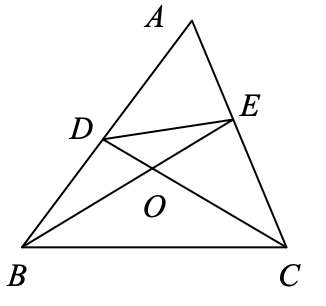
\includegraphics[width=4cm]{picture/6125.png}
\caption{三等角四边形}
\end{figure}
\clearpage
\section{平行四边形基础}
\begin{table}[H]
\centering
\caption{平行四边形的定义、判定与性质}
\begin{tabular}{|l|l|}
\hline
    & 描述 \\
\hline
定义 & 两组对边互相平行的四边形是平行四边形 \\
\hline
判定 & 两组对边分别相等的四边形是平行四边形 \\
\hline
判定 & 一组对边平行且相等的四边形是平行四边形 \\
\hline
判定 & 两组对角分别相等的四边形是平行四边形 \\
\hline
判定 & 对角线互相平分的四边形是平行四边形 \\
\hline
性质 & 平行四边形对边相等 \\
\hline
性质 & 平行四边形对角相等 \\
\hline
性质 & 平行四边形的两条对角线互相平分 \\
\hline
性质 & 平行四边形是中心对称图形,对称中心是两条对角线的交点 \\
\hline
推论 & 夹在两条平行线间的平行线段相等 \\
\hline
\end{tabular}
\end{table}
\begin{problem}
    已知平行四边形两条对角线分别为$m,n$,求平行四边形边长的取值范围。
\end{problem}
\begin{problem}
    已知平行四边形边长和一条对角线分别为$m,n$,求平行四边形另一条对角线的取值范围。
\end{problem}
\begin{problem}
    如图,平行四边形$ABCD,AE\perp BC$于$E$,$AE,BD$相交于$G$,且$DG=2AB,\angle DBC=25^\circ$,求$\angle C$的度数。
\end{problem}
\begin{figure}[H]
\centering
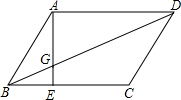
\includegraphics[width=4cm]{picture/603.png}
\caption{练习图}
\end{figure}
\begin{problem}
    如图,在平行四边形$ABCD$中,以$BE$为折痕将$\triangle ABC$向上翻折使得$A$落在$CD$上。
    若$\triangle FDE$周长为8,$\triangle FCB$周长为22,求$FC$的长。
\end{problem}
\begin{problem}
    如图,在等边$\triangle ABC$中,$AB=8$,点$D$在$BC$上,$\triangle ADE$为等边三角形,点$E,D$在直线$AC$两侧。
    过$E$点作$EF\px\px BC$,$EF$与$AB,AC$分别交于$F,G$ \\
    (1)求证:$BF=CE$ \\
    (2)若$AD=7$,求$FG$的长。\\
\end{problem}
\begin{figure}[ht]
\begin{minipage}[t]{0.48\textwidth}
\centering
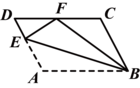
\includegraphics[width=4cm]{picture/6_2_1.png}
\caption{练习图}
\end{minipage}
\begin{minipage}[t]{0.48\textwidth}
\centering
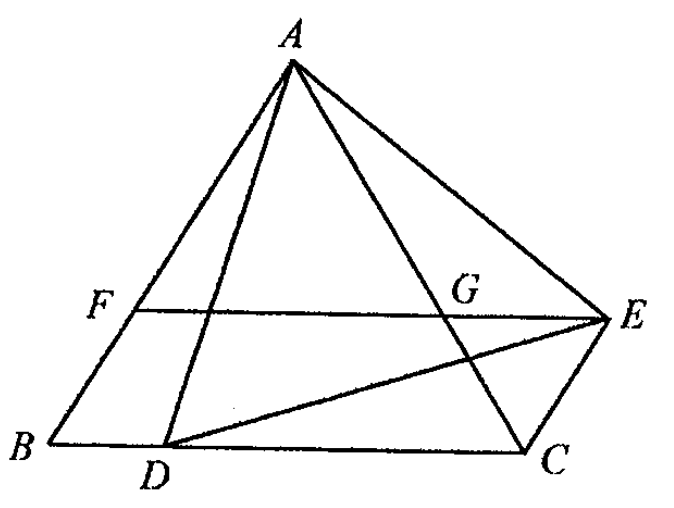
\includegraphics[width=4cm]{picture/6_2_2.png}
\caption{练习图}
\end{minipage}
\end{figure}
\begin{problem}
    如图,$\triangle ABC$分别以$AB,AC,BC$为边在$BC$同侧作三个等边三角形,探究$\triangle ABC$满足什么条件时,以下结论成立:\\
    (1)四边形$DAEF$为矩形 \\
    (2)四边形$DAEF$为菱形 \\
    (3)以$D,A,E,F$为顶点的四边形不存在
\end{problem}
\begin{figure}[H]
\centering
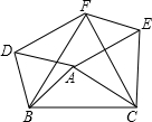
\includegraphics[width=4cm]{picture/671.png}
\caption{练习图}
\end{figure}
\begin{problem}
    如图,菱形$ABCD$中,点$E,F$分别在边$BC,CD$上,$\angle BAF=\angle DAE$,$AE,BD$交于$G$. \\
    (1)求证:$EF\px \px BD$. \\
    (2)当$BE=GF$时,求证:四边形$BEFG$为平行四边形. \\
\end{problem}
\begin{figure}[H]
\centering
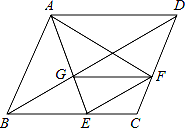
\includegraphics[width=4cm]{picture/6127.png}
\caption{练习图}
\end{figure}
\begin{problem}
    如图,平行四边形$ABCD,AB=5,BC=4,AC=\sqrt{17},\triangle ABC$的平分线交$CD$于$E$,交$AC$于$F$. \\
    (1)求平行四边形$ABCD$面积。\\
    (2)若$P$为$BC$上一动点(不与$B,C$重合),连$EP$,设$BP=x,S_{\triangle PFC}=y$,求$y$关于$x$的函数解析式,并写出定义域。\\
\end{problem}
\begin{figure}[H]
\centering
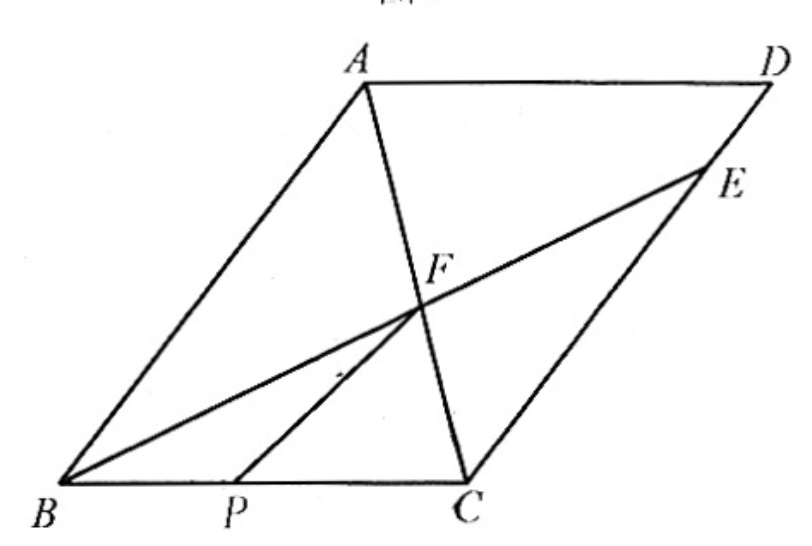
\includegraphics[width=4cm]{picture/6130.png}
\caption{练习图}
\end{figure}
\clearpage
\section{平行四边形的坐标}
\begin{conclusion}
    在平行四边形$ABCD$中,$A(x_1,y_1),B(x_2,y_2),C(x_3,y_3),D(x_4,y_4)$,则有如下结论成立: \\
    (1)对称中心$O$点坐标为$(\frac{x_1+x_3}{2},\frac{y_1+y_3}{2})$或$(\frac{x_2+x_4}{2},\frac{y_2+y_4}{2})$ \\
    (2)$x_1+x_3=x_2+x_4,y_1+y_3=y_2+y_4$ \\
\end{conclusion}
\begin{problem}
    如图,在菱形$ABCD$中,$A(0,4),C(0,-12),F(3,0)$,求$B$点坐标。
\end{problem}
\begin{figure}[H]
\centering
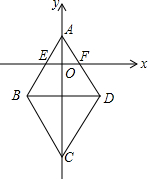
\includegraphics[width=4cm]{picture/646.png}
\caption{练习图}
\end{figure}
\begin{problem}
    如图,直线$l_1:y_1=-3x+3$与$x$轴交于$D$点,另一直线$l_2:y_2=kx+b$经过$A,B$两点,与$l_1$交于点$D$。
    直接写出$E$点坐标,使得以$E,A,C,D$为顶点的四边形为平行四边形。
\end{problem}
\begin{figure}[H]
\centering
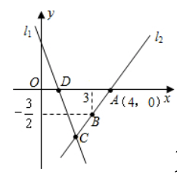
\includegraphics[width=4cm]{picture/667.png}
\caption{练习图}
\end{figure}
\begin{problem}
    如图,四边形$ABCD$为平行四边形,$BC=2AB,A(-1,0),B(0,2),C,D$在反比例函数$y=\frac{k}{x}(k<0)$上,求$k$的值。
\end{problem}
\begin{figure}[H]
\centering
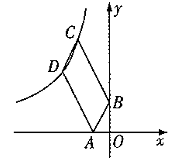
\includegraphics[width=4cm]{picture/670.png}
\caption{练习图}
\end{figure}
\begin{problem}
    如图,直线$y=mx+4$与反比例函数$y=\frac{k}{x}(k>0)$图像交于$A,B$两点,与$x$轴负半轴,$y$轴交于$D,C$两点,$CO:DO=2$,$D$,$A$点横坐标为1.
    点$M$在直线$x=-1$上,点$N$在反比例函数上,若以$A,B,M,N$为顶点的四边形是平行四边形,求点$N$的坐标。
\end{problem}
\begin{figure}[H]
\centering
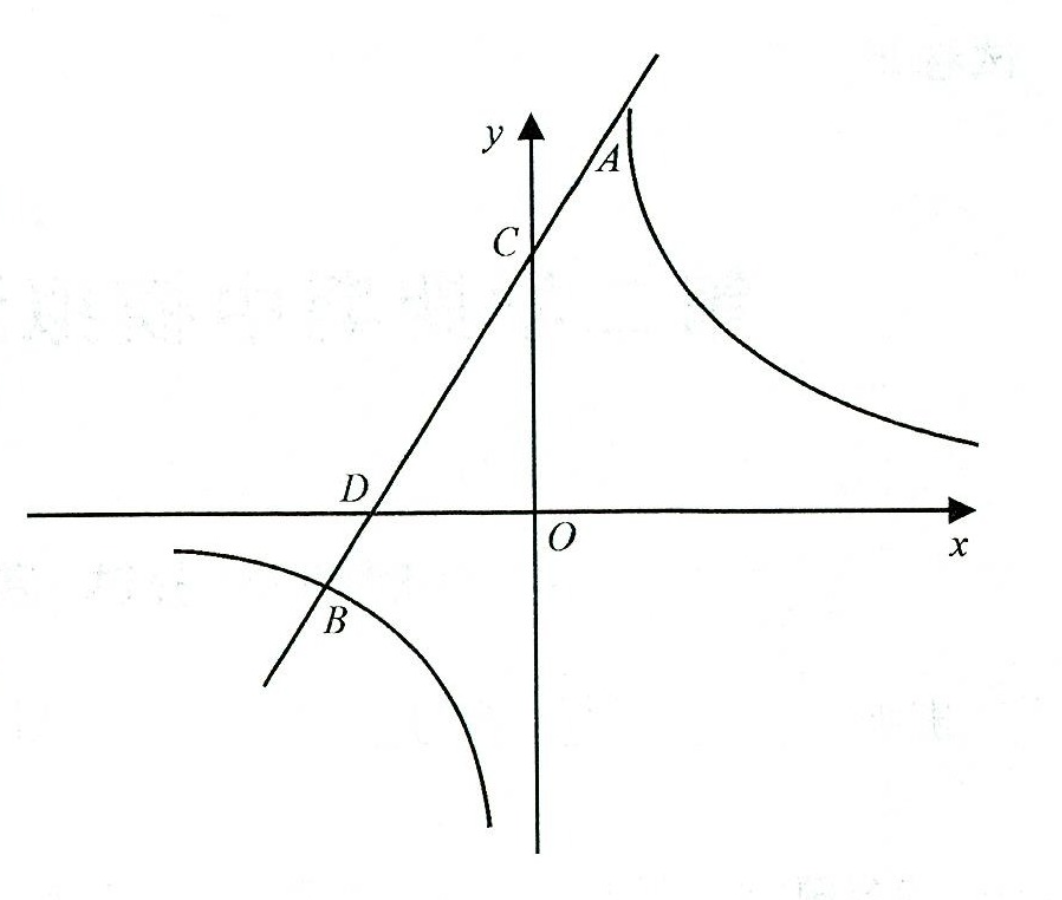
\includegraphics[width=4cm]{picture/6123.png}
\caption{练习图}
\end{figure}
\clearpage
\section{平行四边形的对称中心}
\begin{model}
    如图,平行四边形$ABCD$中,$O$为两条对角线交点,$EF$过点$O$分别交$AD,BC$于$E,F$,有如下结论成立:\\
    (1)$EF$平分$ABCD$周长和面积 \\
    (2)$OF=OE$ \\
    (3)$S_{\triangle ABO}=S_{\triangle ADO}=S_{\triangle BCO}=S_{\triangle CDO}$ \\
    (4)若一条直线平分平行四边形面积,则该直线一定经过平行四边形对称中心
\end{model}
\begin{figure}[H]
\centering
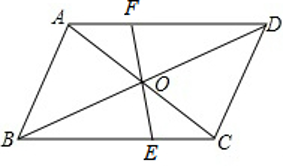
\includegraphics[width=4cm]{picture/668.png}
\caption{练习图}
\end{figure}
\begin{problem}
    如图,$AB\px\px DC \px\px EF,AD\px\px CF\px\px BE$,请画出一条直线,平分该多边形的面积。
\end{problem}
\begin{figure}[H]
\centering
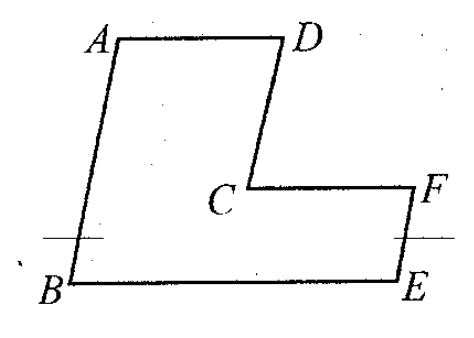
\includegraphics[width=4cm]{picture/6_2_3.png}
\caption{练习图}
\end{figure}
\begin{problem}
    如图,平行四边形$ABCO,A(5,0),C(1,4)$,过点$P(0,-2)$的直线交平行四边形于$M,N$两点,且将平行四边形分成面积相等的两部分,求$MN$的长度。
\end{problem}
\begin{figure}[H]
\centering
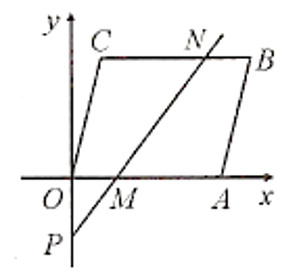
\includegraphics[width=4cm]{picture/669.png}
\caption{练习图}
\end{figure}
\clearpage
\section{面积问题}
\begin{model}
    与平行四边形等底等高的三角形面积是平行四边形的一半。\\
    如图,可以分析出$S_1=S_2$
\end{model}
\begin{figure}[H]
\centering
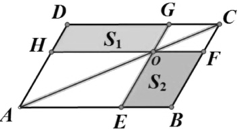
\includegraphics[width=3cm]{picture/680.png}
\caption{等面积模型}
\end{figure}
\begin{model}
    如图,平行四边形$ABCD$,$P$为平行四边形内一点,则有$S_{\triangle ABP}+S_{\triangle CDP}=S_{\triangle ADP}+S_{\triangle BCP}.$
\end{model}
\begin{figure}[H]
\centering
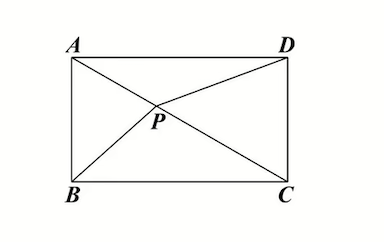
\includegraphics[width=4cm]{picture/6115.png}
\caption{等面积模型}
\end{figure}
\begin{problem}
    如图,在平行四边形$ABCD$中,$E$为$AD$上一点,$F$为$AB$上一点。$BE,DF$交于点$G$且$BE=DF$,连$GC$,求证:$GC$平分$\angle BGD$
\end{problem}
\begin{figure}[H]
\centering
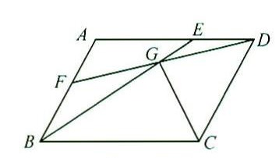
\includegraphics[width=3cm]{picture/681.png}
\caption{练习图}
\end{figure}
\begin{problem}
    如图,在平行四边形$𝐴𝐵𝐶𝐷$中,$𝐸,F,𝑄,𝑃$分别为$𝐴𝐷,𝐷𝐶,𝐶𝐵,𝐵𝐴$的中点,若平行四边形$𝐴𝐵𝐶𝐷$面积为4,求$\triangle𝑃𝑄𝑇$的面积。
\end{problem}
\begin{figure}[H]
\centering
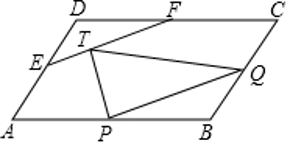
\includegraphics[width=3cm]{picture/682.png}
\caption{练习图}
\end{figure}
\begin{problem}
    如图,平行四边形$𝐴𝐵𝐶𝐷$的面积为64,$E,F$分别为$AB,AC$中点,求$\triangle CEF$的面积。
\end{problem}
\begin{figure}[H]
\centering
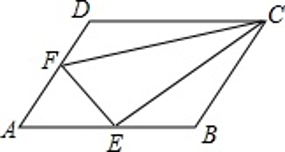
\includegraphics[width=3cm]{picture/683.png}
\caption{练习图}
\end{figure}
\begin{problem}
    如图,过平行四边形$𝐴𝐵𝐶𝐷$内一点$P$作边的平行线$EF,GH$,若阴影部分面积为$8$,则平行四边形$PHCF$面积比平行四边形$PGAE$大多少?
\end{problem}
\begin{figure}[H]
\centering
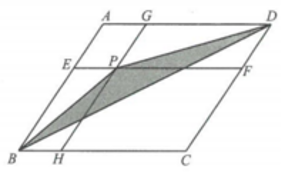
\includegraphics[width=4cm]{picture/684.png}
\caption{练习图}
\end{figure}
\begin{problem}
    如图,平行四边形$ABCD$的面积为120,$E$为$AB$上一点,且$AE=2BE$,$DE,CB$延长线交于$F$,求$\triangle AEF$与$\triangle BCE$的面积和。
\end{problem}
\begin{figure}[H]
\centering
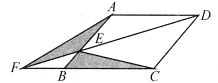
\includegraphics[width=4cm]{picture/687.png}
\caption{练习图}
\end{figure}
\clearpage
\section{矩形基础}
\begin{knowledge}
    如图,矩形$ABCD$,对角线$AC,BD$交于点$O$,则有如下结论成立:\\
    (1)$OA=OB=OC=OD$ \\
    (2)若$\angle ACB=30^\circ$,则$\triangle ABO,\triangle CDO$为等边三角形 \\
\end{knowledge}
\begin{figure}[H]
\centering
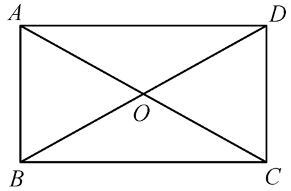
\includegraphics[width=4cm]{picture/653.png}
\caption{矩形}
\end{figure}
\begin{table}[H]
\centering
\caption{矩形的定义、判定与性质}
\begin{tabular}{|l|l|}
\hline
    & 描述 \\
\hline
定义 & 有一个角是直角的平行四边形是矩形 \\
\hline
判定 & 有三个角是直角的四边形是矩形 \\
\hline
判定 & 对角线相等的平行四边形是矩形 \\
\hline
性质 & 矩形四个角都是直角 \\
\hline
性质 & 矩形对角线相等 \\
\hline
对称性 & 矩形是轴对称图形,2条对称轴,对称轴为对边中点连线 \\
\hline
\end{tabular}
\end{table}
\begin{problem}
    如图,矩形$ABCD$中,$AB=2AD$,$E$是$CD$的中点,且$AB=AF$,求$\angle EBF$.
\end{problem}
\begin{figure}[H]
\centering
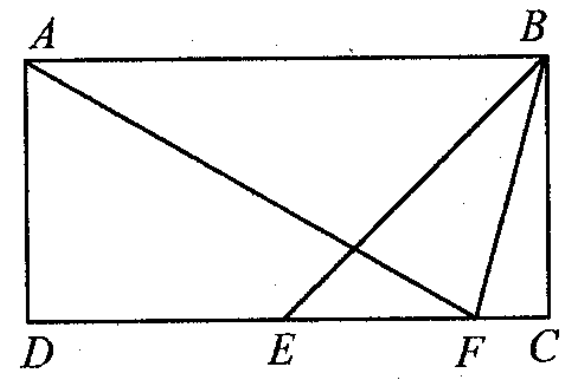
\includegraphics[width=4cm]{picture/688.png}
\caption{练习图}
\end{figure}
\begin{problem}
    如图,点$E,F$分别是平行四边形$ABCD$边$AD,BC$的中点,$AD=2AB$,连$AC,BE$交于$G$,$DF,CE$交于$H$,求证:四边形$EGFH$为矩形。
\end{problem}
\begin{figure}[H]
\centering
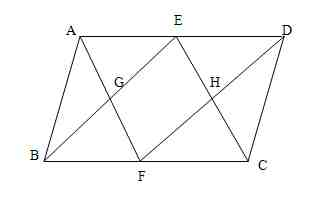
\includegraphics[width=4cm]{picture/605.jpeg}
\caption{练习图}
\end{figure}
\begin{problem}
    如图,$P$为$\triangle ABC$边$BC$上一动点,$MN\px\px BC$交$\angle BCA$平分线于点$E$,交$\angle BCA$外角平分线于点$F$。\\
    (1)求证:$PE=PF$ \\
    (2)当$P$运动到何处时,四边形$AECF$为矩形? \\
    (3)若四边形$AECF$为正方形,且$\frac{AP}{BC}=\frac{\sqrt{3}}{2}$,求$\angle BAC$ \\
\end{problem}
\begin{figure}[H]
\centering
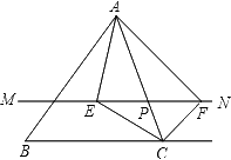
\includegraphics[width=4cm]{picture/654.png}
\caption{练习图}
\end{figure}
\begin{problem}
    如图,等腰梯形$ABCD$中,$AB\px \px CD,AD=BC$,对角线$AC,BD$交于$O$,$E,F$分别在$OA,OB$上,$OC=OE,OD=OF$,求证:四边形$DEFC$为矩形。
\end{problem}
\begin{figure}[H]
\centering
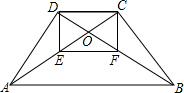
\includegraphics[width=4cm]{picture/6_3_2.png}
\caption{练习图}
\end{figure}
\begin{problem}
    如图,点$P$是平行四边形$ABCD$外一点。\\
    (1)若四边形$ABCD$为矩形,$PA\perp PC$,求证:$PB\perp PD$。 \\
    (2)若$PA \perp PC,PB \perp PD$,求证:四边形$ABCD$为矩形。 \\
\end{problem}
\begin{figure}[H]
\centering
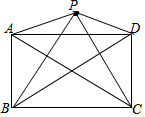
\includegraphics[width=4cm]{picture/639.png}
\caption{练习图}
\end{figure}
\begin{problem}
    如图,$BE,BD$分别是$\angle ABC$的内外角平分线,$AD\perp BD,AE\perp BE$交$BC$延长线于$F$,求证:$DE=BF$。 \\
\end{problem}
\begin{figure}[H]
\centering
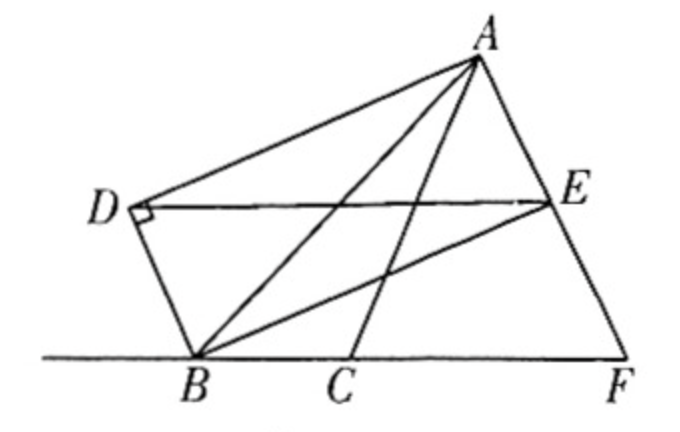
\includegraphics[width=4cm]{picture/641.png}
\caption{练习图}
\end{figure}
\clearpage
\section{腰双高模型}
\begin{problem}
    如图,$\triangle ABC,\angle C=90^\circ,PE\perp BD,PF\perp AD,BD=AD$,求证:$PE+PF=BC$
\end{problem}
\begin{figure}[H]
\centering
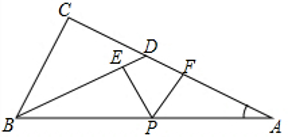
\includegraphics[width=3cm]{picture/655.png}
\caption{练习图}
\end{figure}
\begin{problem}
    如图,矩形$ABCD$中,将$\triangle BCD$沿着$BD$翻折,$AB=2,PN\perp BE,PM\perp AD$,求$PN+PM$的值。
\end{problem}
\begin{figure}[H]
\centering
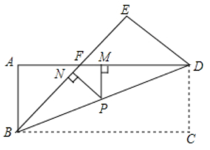
\includegraphics[width=3cm]{picture/656.png}
\caption{练习图}
\end{figure}
\begin{problem}
    如图,矩形$ABCD$中,$AB=3,BC=4,PE\perp AC, PF\perp BD$,求$PE+PF$的值。
\end{problem}
\begin{figure}[H]
\centering
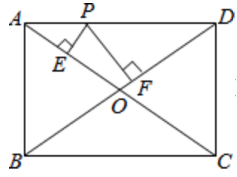
\includegraphics[width=3cm]{picture/657.png}
\caption{练习图}
\end{figure}
\begin{problem}
    如图,正方形$ABCD$边长为1,$BE=BC,PM\perp BE, PN\perp BC$,求$PM+PN$的值。
\end{problem}
\begin{figure}[H]
\centering
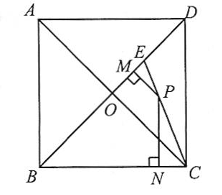
\includegraphics[width=3cm]{picture/658.png}
\caption{练习图}
\end{figure}
\clearpage
\section{翻折问题}
\begin{model}
    如图,将矩形$ABCD$沿着对角线$BD$翻折,$C$点翻折到$E$点,则四边形$ABDE$为等腰梯形。
\end{model}
\begin{figure}[H]
\centering
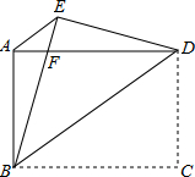
\includegraphics[width=4cm]{picture/672.png}
\caption{练习图}
\end{figure}
\begin{problem}
    如上图,若$AB=6,BC=8$. \\
    (1)求证:四边形$ABDE$为等腰梯形. \\
    (2)求四边形$BCDF$的周长. \\
    (3)求四边形$ABDE$的面积.
\end{problem}
\begin{model}
    如图,平行四边形$ABCD$,将$\triangle ABC$沿着$AC$翻折,$B$点翻折到$B'$,则$\triangle BB'D$为直角三角形。\\
\end{model}
\begin{figure}[H]
\centering
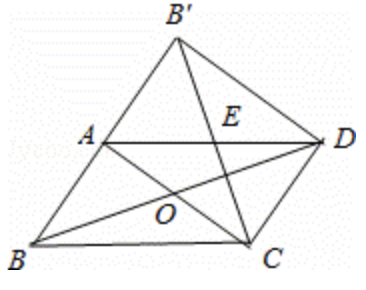
\includegraphics[width=4cm]{picture/6131.png}
\caption{模型图}
\end{figure}
\begin{problem}
    平行四边形$ABCD$,$AC,BD$交于点$O,\angle AOB=60^\circ,BD=4$,将$\triangle ABC$沿直线$AC$翻折,点$B$落在点$E$,求$S_{\triangle AED}$.
\end{problem}
\begin{problem}
    如图,矩形$ABCD$中,$E$为边$AB$的中点,将$\triangle EBC$沿着$EC$翻折,点$B$落在$P$处,连$BP$交$CE$于$Q$. \\
    (1)求证:四边形$AECF$为平行四边形。\\
    (2)若$PA=PE$,求证:$\triangle APB \backcong \triangle EPC$.
\end{problem}
\begin{figure}[H]
\centering
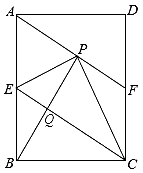
\includegraphics[width=4cm]{picture/6121.png}
\caption{练习图}
\end{figure}
\begin{model}
    如图,矩形$ABCD$沿着直线$EF$折叠,$B$的对称点$B'$恰好与$D$重合,则有四边形$BEDF$为菱形,四边形$AA'B'B$为等腰梯形。
\end{model}
\begin{figure}[H]
\centering
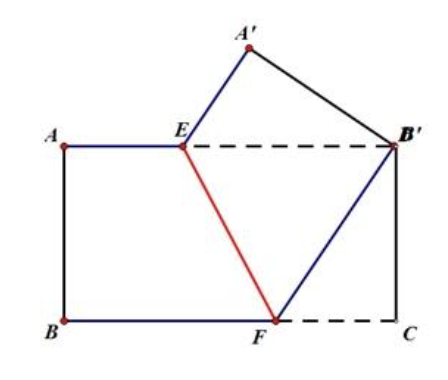
\includegraphics[width=4cm]{picture/6132.png}
\caption{模型图}
\end{figure}
\begin{problem}
    将矩形$ABCD$沿某条直线折叠,使得对角线两个端点$A,C$重合,折叠所在直线交射线$AB$于点$E$,若$AB=3,BE=1$,求$BC$的长。
\end{problem}
\begin{problem}
    矩形$ABCD$中,$AB=6,AD=8$,$E$为$BC$上的点,以$AE$为折痕折叠,$B$落在$F$。连接$FC$,若$\triangle EFC$为直角三角形,求$BE$的长度。
\end{problem}
\begin{problem}
    如图,矩形纸片$ABCD$,$AB=3,AD=5$,翻折纸片使得$A$落在$BC$上$E$处,折痕为$PQ$。$E$在边$BC$上移动时,折痕端点$P,Q$也随之移动,
    若限定$P,Q$分别在$AB,AD$上移动,求$E$在$BC$上可移动的最大距离。
\end{problem}
\begin{figure}[H]
\centering
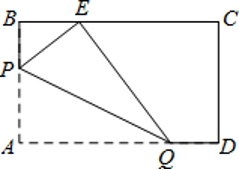
\includegraphics[width=4cm]{picture/676.png}
\caption{练习图}
\end{figure}
\clearpage
\section{四边形与勾股定理}
\begin{conclusion}
    平行四边形$ABCD$满足$2AB^2+2BC^2=AC^2+BD^2$.
\end{conclusion}
\begin{corollary}
    菱形两条对角线的平方和等于菱形一边长平方和的4倍。
\end{corollary}
\begin{figure}[H]
\centering
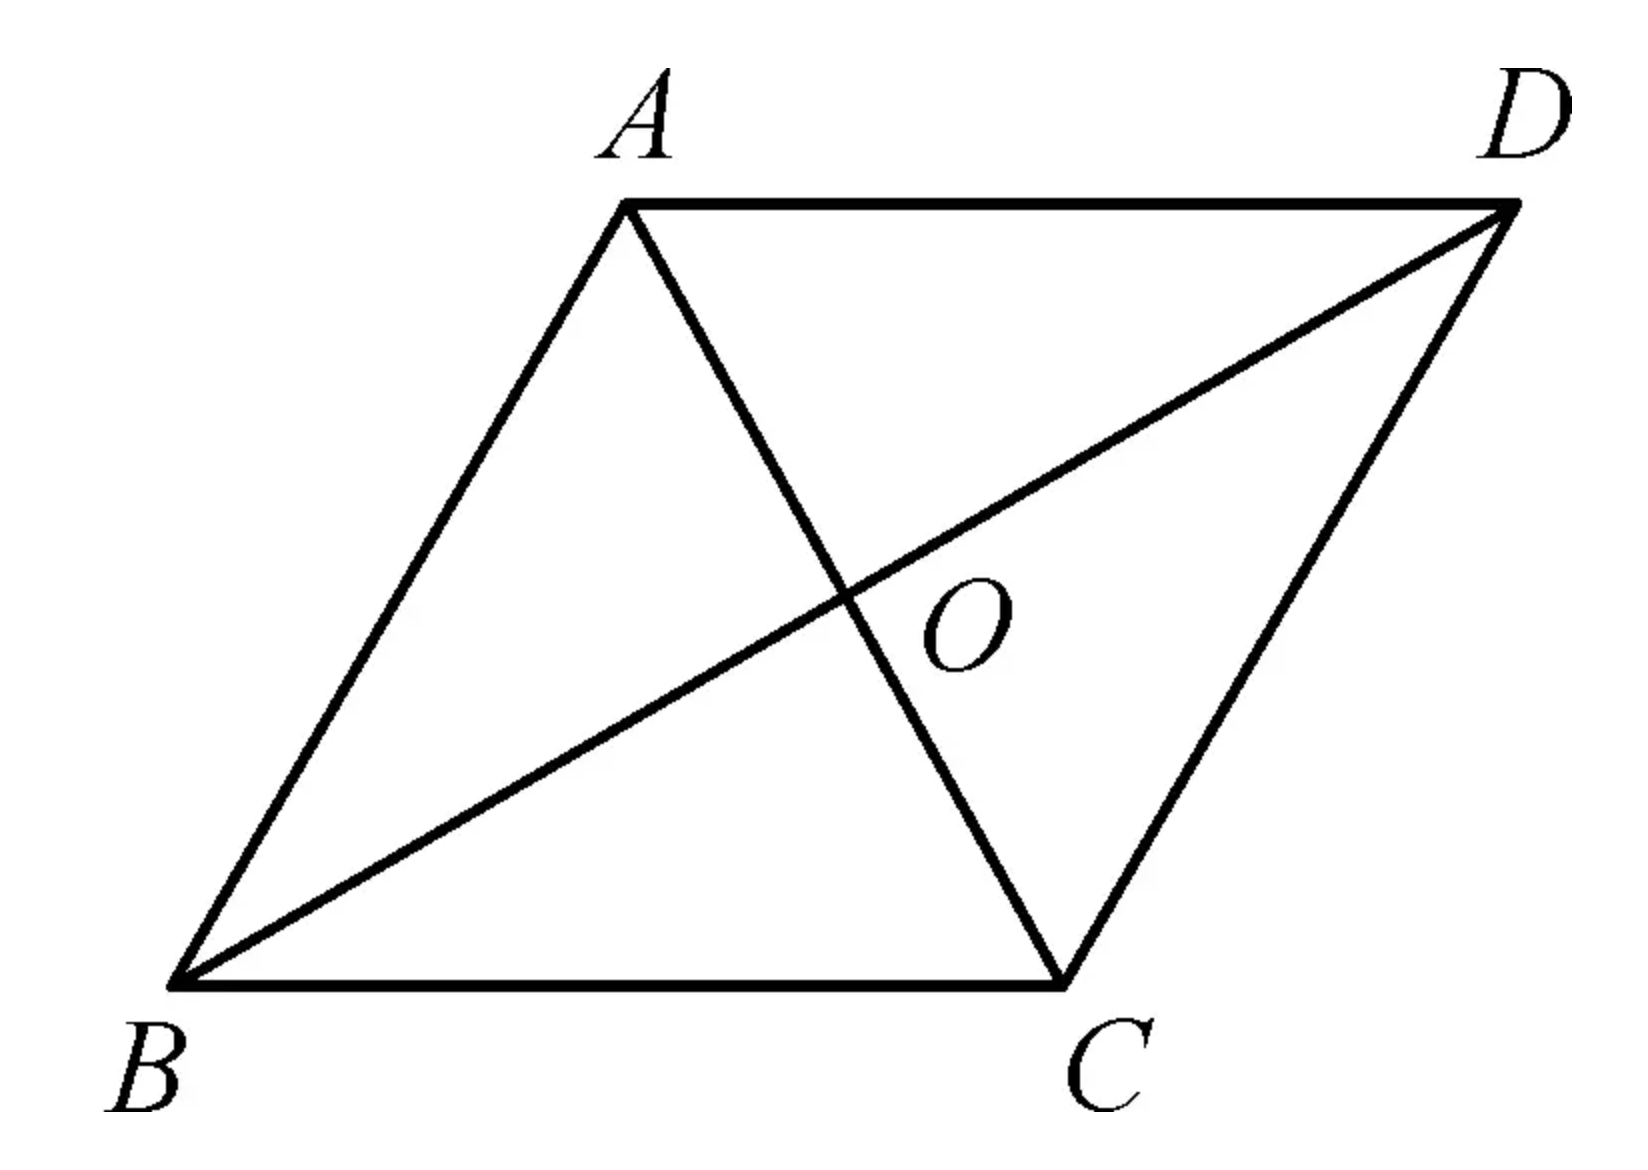
\includegraphics[width=4cm]{picture/606.png}
\caption{菱形}
\end{figure}
\begin{model}
    如图,矩形$ABCD$,$P$为平面内一点,则有结论$PA^2+PC^2=PB^2+PD^2$成立。
\end{model}
\begin{figure}[H]
\centering
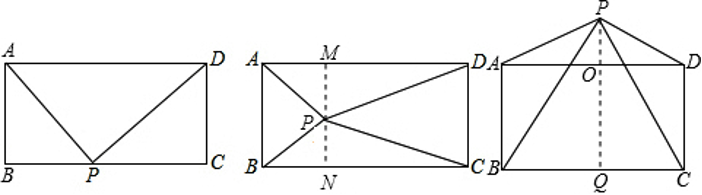
\includegraphics[width=8cm]{picture/660.png}
\caption{矩形勾股定理}
\end{figure}
\begin{model}
    如图,四边形$ABCD$对角线垂直,有如下结论成立: \\
    (1)$S_{ABCD}=\frac{1}{2}AC·BD$ \\
    (2)$AB^2+CD^2=AD^2+BC^2$ \\
    (3)中点四边形$EFGH$为矩形
\end{model}
\begin{figure}[H]
\centering
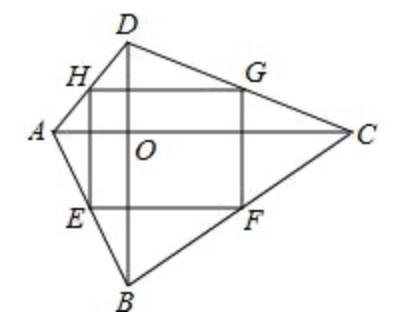
\includegraphics[width=4cm]{picture/665.png}
\caption{对角线垂直的四边形}
\end{figure}
\begin{problem}
    如图,矩形$ABCD$,$P$在对角线$AC$上,过点$P$作$EF\px\px AB$,分别交$AB,CD$于点$E,F$,连$PB,PD$。
    若$PB=2\sqrt5,PD=6$,阴影部分面积为9,求矩形$ABCD$的周长。
\end{problem}
\begin{figure}[H]
\centering
\includegraphics[width=4cm]{picture/661.png}
\caption{练习图}
\end{figure}
\begin{problem}
    如图1,我们把对角线互相垂直的四边形叫做垂美四边形。 \\
    (1)图2是一个特殊的四边形,满足$AD=AB,CD=CB$,证明四边形$ABCD$为垂美四边形。\\
    (2)证明:对于任意的垂美四边形,对边的平方和相同,即$AD^2+BC^2=AB^2+CD^2$。 \\
    (3)如图3,分别以直角三角形$ABC$的直角边$AC$和斜边$AB$为边外作正方形$ACFG$和正方形$ABDE$,连接$CE,BG,GE$。若$AC=4,AB=5$,求$GE$的长度。
\end{problem}
\begin{figure}[H]
\centering
\includegraphics[width=6cm]{picture/666.png}
\caption{练习图}
\end{figure}
\clearpage
\section{菱形基础}
\begin{table}[H]
\centering
\caption{菱形的定义、判定与性质}
\begin{tabular}{|l|l|}
\hline
    & 描述 \\
\hline
定义 & 有一组邻边相等的平行四边形是菱形 \\
\hline
判定 & 四条边都相等的四边形是菱形 \\
\hline
判定 & 对角线互相垂直的平行四边形是菱形 \\
\hline
性质 & 菱形四条边都相等 \\
\hline
性质 & 菱形对角线互相垂直,每条对角线平分一组对角 \\
\hline
对称性 & 菱形是轴对称图形,2条对称轴,对称轴为对角线所在直线 \\
\hline
\end{tabular}
\end{table}
\begin{problem}
    菱形$ABCD$的边长为$a$,两条对角线的和为$b$,求菱形的面积。
\end{problem}
\begin{problem}
    将两张宽度相等的矩形纸片叠放在一起得到如图5所示的四边形$ABCD$. \\
    (1)判断四边形$ABCD$的形状,并证明。 \\
    (2)若矩形的长为8,宽为2,求四边形$ABCD$周长的最小值和最大值。 \\
\end{problem}
\begin{figure}[H]
\centering
\includegraphics[width=4cm]{picture/607.png}
\caption{练习图}
\end{figure}
\begin{problem}
    如图,在$\triangle ABC$中,$BC$上有一点$P$,过$P$分别作$AB,AC$平行线,分别交$AB,AC$于点$E,D$。作出点$P$,使得四边形$AEPD$为菱形并证明。
\end{problem}
\begin{figure}[H]
\centering
\includegraphics[width=4cm]{picture/635.jpg}
\caption{练习图}
\end{figure}
\begin{problem}
    如图,在$\triangle ABC$中,点$D,E$分别是边$AB,BC$的中点,点$F,G$是边$AC$的三等分点,$DF,EG$的延长线相交于点$H$ \\
    (1)求证:四边形$FBGH$是平行四边形 \\
    (2)若$AC$平分$\angle BAH$,求证:四边形$ABCH$为菱形 \\
\end{problem}
\begin{figure}[H]
\centering
\includegraphics[width=4cm]{picture/678.png}
\caption{练习图}
\end{figure}
\begin{problem}
    如图,在$\triangle ABC$中,$\angle ACB=90^\circ$,$CD$为$AB$边上的高,$\angle BAC$的平分线$AE$交$CD$于$F$,$EG\perp AB$于$G$,
    求证:四边形$GECF$是菱形。
\end{problem}
\begin{figure}[H]
\centering
\includegraphics[width=4cm]{picture/679.png}
\caption{练习图}
\end{figure}
\clearpage
\section{内角为$60^\circ$的菱形}
\begin{model}
    如图,菱形$ABCD$中,$\angle B=60^\circ,E,F$为$BC,CD$上的动点,且满足$\angle EAF=60^\circ$.设$AB=a$,有如下结论成立:\\
    (1)$\triangle AEB \backcong \triangle AFC \sim \triangle AGF \sim \triangle EGC$ \\
    (2)$\triangle AEC \backcong \triangle AFD \sim \triangle AGE \sim \triangle FGC$ \\
    (3)$\triangle EAF$为等边三角形 \\
    (4)四边形$AECF$的面积为$\frac{\sqrt3}{4}a^2$ \\
    (5)菱形的面积为$\frac{\sqrt3}{2}a^2$ \\
    (6)$AC=a,BD=\sqrt3a$
\end{model}
\begin{figure}[H]
\centering
\includegraphics[width=4cm]{picture/608.png}
\caption{含60度角的菱形}
\end{figure}
\begin{problem}
    已知菱形有一个内角为$60^\circ$,一条对角线长为$4\sqrt3$,求菱形的面积。
\end{problem}
\begin{problem}
    如图,菱形$ABCD,AB=6,\angle A=60^\circ$,$E$为线段$AB$上不与$A,B$重合的一点. \\
    (1)作$EDF=60^\circ$交$BC$于$F$,求证:$\triangle DEF$为等边三角形\\
    (2)在(1)的基础上,探究四边形$DEBF$周长的最小值 \\
    (3)作$DEF=60^\circ$交$BC$于$F$,(1)中结论是否依然成立?若成立请证明,不成立请说明理由 \\
\end{problem}
\begin{figure}[H]
\centering
\includegraphics[width=4cm]{picture/609.png}
\caption{练习图}
\end{figure}
\begin{problem}
    如图,菱形$ABCD$中,$AC=2,\angle B=60^\circ$.$E$为线段$BC$上一点,且不与$B,C$重合,作$\angle EAF=60^\circ$交$CD$于$F$.设$CE=x,EG=y$.\\
    (1)证明:$\triangle AEF$为等边三角形。 \\
    (2)求$y$关于$x$的函数解析式,并写出定义域。 \\
    (3)设点$O$为线段$AC$中点,若$EG=EO$,求$x$的值。 \\
\end{problem}
\begin{figure}[H]
\centering
\includegraphics[width=4cm]{picture/609.png}
\caption{练习图}
\end{figure}
\begin{problem}
    如图,菱形$ABCD$边长为2,$\angle B=60\circ$,$M$为边$AB$中点,$N$为边$BC$上一动点(不与$B$重合),
    将$\triangle BMN$沿着直线$MN$折叠,点$B$落在点$E$处,连$DE,CE$. \\
    (1)当$N$为$BC$中点时,求$CE$的长。\\
    (2)当$\triangle CDE$为等腰三角形时,求$BN$的长。
\end{problem}
\begin{figure}[H]
\centering
\includegraphics[width=6cm]{picture/6124.png}
\caption{练习图}
\end{figure}
\begin{problem}
    如图,平行四边形$ABCD$,$P$为对角线$BD$上一个动点,且不与$BD$中点重合,$PA=OC$.\\
    (1)求证:四边形$ABCD$为菱形。\\
    (2)若$AB=6,\angle ABC=60^\circ$,设$BP=x,AP=y$,求$y$关于$x$的函数解析式,并写出定义域。\\
    (3)在(2)的条件下,延长$AP$交射线$BC$于点$E$,当$\triangle EPC$为直角三角形时,求$BP$的长。 \\
\end{problem}
\begin{figure}[H]
\centering
\includegraphics[width=6cm]{picture/6128.png}
\caption{练习图}
\end{figure}
\clearpage
\section{正方形基础}
\begin{table}[H]
\centering
\caption{正方形的定义、判定与性质}
\begin{tabular}{|l|l|}
\hline
    & 描述 \\
\hline
定义 & 一组邻边相等且垂直的平行四边形是四边形 \\
\hline
判定 & 一组邻边相等的矩形是正方形 \\
\hline
判定 & 有一个角为直角的菱形是正方形 \\
\hline
性质 & 正方形四条边相等,四个角都是直角 \\
\hline
性质 & 正方形对角线相等且互相垂直平分 \\
\hline
对称性 & 正方形是轴对称图形,有4条对称轴\\
\hline
\end{tabular}
\end{table}
\begin{problem}
    如图,平行四边形$ABCD$的四条内角平分线围成四边形$GEHF$. \\
    (1)判断四边形$GEHF$的形状,并证明。\\
    (2)若四边形$ABCD$为矩形,判断四边形$GEHF$的形状,并证明。\\
\end{problem}
\begin{figure}[H]
\centering
\includegraphics[width=4cm]{picture/6120.png}
\caption{练习图}
\end{figure}
\begin{problem}
    如图,边长为6的正方形$ABCD$中有两个小正方形,求这两个小正方形的面积之和。
\end{problem}
\begin{figure}[H]
\centering
\includegraphics[width=4cm]{picture/644.png}
\caption{练习图}
\end{figure}
\begin{problem}
    如图,直角三角形$ACB,\angle C=90^\circ$,$\angle A,\angle B$的平分线交于点$D,DE\perp BC$于$E,DF\perp AC$于$F$,
    求证:四边形$CEDF$为正方形.
\end{problem}
\begin{figure}[H]
\centering
\includegraphics[width=4cm]{picture/6118.png}
\caption{练习图}
\end{figure}
\begin{problem}
    如图,点$A',B',C',D'$是正方形$ABCD$四边上的一点,满足$AA'=BB'=CC'=DD'$。\\
    (1)求证:四边形$A'B'C'D'$为正方形。 \\
    (2)探究当$A',B',C',D'$位于什么位置时,正方形$A'B'C'D'$为正方形$ABCD$面积的$\frac{5}{9}$. \\
\end{problem}
\begin{figure}[H]
\centering
\includegraphics[width=4cm]{picture/643.png}
\caption{练习图}
\end{figure}
\clearpage
\section{旋转模型}
\begin{model}
    如图,以下四个图形中,$CD=CB,\angle DAB=\alpha,\angle DCB=\beta$.\\
    (1)$\alpha=90^\circ,\beta=90^\circ\Rightarrow AD+AB=\sqrt2 AC$ \\
    (2)$\alpha=90^\circ,\beta=90^\circ\Rightarrow AB-AD=\sqrt2 AC$ \\
    (3)$\alpha=60^\circ,\beta=120^\circ\Rightarrow AD+AB=\sqrt3 AC$ \\
    (4)$\alpha=60^\circ,\beta=120^\circ\Rightarrow AB-AD=\sqrt3 AC$ \\
\end{model}
\begin{figure}[H]
\centering
\includegraphics[width=12cm]{picture/6108.png}
\caption{旋转模型}
\end{figure}
\begin{model}
    如图,正方形$ABCD$中,$AC,BD$交于$O$,$E$为$AB$上一点,$F$为$BC$上一点且$OE\perp OF$,有如下结论成立:\\
    (1)$\triangle BEO \backcong \triangle CFO$ \\
    (2)$OE=OF,\triangle EOF$为等腰直角三角形 \\
    (3)四边形$BEOF$面积为定值,且为正方形$ABCD$面积的$\frac{1}{4}$ \\
    (4)$BE+BF=\sqrt2 OB$ \\
    (5)$CF^2+BF^2=2OF^2$ \\
\end{model}
\begin{figure}[H]
\centering
\includegraphics[width=3cm]{picture/6109.png}
\caption{旋转模型}
\end{figure}
\begin{problem}
    如图,$n$个边长为1的正方形按照图示摆放,$A_1,A_2,…,A_n$分别是正方形的中心,求$n$个正方形重叠后阴影部分的面积。
\end{problem}
\begin{figure}[H]
\centering
\includegraphics[width=4cm]{picture/6112.png}
\caption{练习图}
\end{figure}
\begin{problem}
    如图,在正方形$ABCD$中,$F$为对角线$AC$上任意一点,$EF\perp BF$交$AD$于$E$,联结$BE$,求$\angle EBF$的度数。\\
\end{problem}
\begin{figure}[H]
\centering
\includegraphics[width=3cm]{picture/645.png}
\caption{练习图}
\end{figure}
\begin{problem}
    如图,正方形$ABCD$边长为6,$AC,BD$交于点$O$,$E$为$CD$上一点,$DE=2CE,CF\perp BE$交$BE$于$F$,求$OF$的长。
\end{problem}
\begin{figure}[H]
\centering
\includegraphics[width=3cm]{picture/6110.png}
\caption{练习图}
\end{figure}
\begin{problem}
    如图,在正方形$ABCD$中,$E$为$AC$上一点,$F$为$CD$上一点,$ED=EF$. \\
    (1)求证:$DF=\sqrt2 AE$ \\
    (2)求证:$BF=\sqrt2 EF$ \\
    (3)求证:$CB+CF=\sqrt2 CE$ \\
\end{problem}
\begin{figure}[H]
\centering
\includegraphics[width=3cm]{picture/6111.png}
\caption{练习图}
\end{figure}
\clearpage
\section{十字架模型}
\begin{model}
    在正方形$ABCD$中 \\
    (1)如左图,$AF\perp BE \Leftrightarrow AF=BE$ \\
    (2)如右图,$MP\perp NQ \Rightarrow MP=NQ$
\end{model}
\begin{figure}[H]
\centering
\includegraphics[width=6cm]{picture/6100.png}
\caption{十字架模型图}
\end{figure}
\begin{problem}
    如图,在正方形$ABCD$中,$E,F$分别为$CD,AD$中点,设正方形边长为$a$. \\
    (1)求证:$BE\perp CF$ \\
    (2)用含$a$的式子表示$AP,CP$的长度
\end{problem}
\begin{figure}[H]
\centering
\includegraphics[width=3cm]{picture/6101.png}
\caption{练习图}
\end{figure}
\begin{problem}
    如图,在正方形$ABCD$中,$E$为$AD$中点,$F$为$CD$上一点,$AF\perp BE$,$M$为$AD$上一点,且满足$BM=DM+CD$. \\
    (1)求证:$CF=FD$ \\
    (2)求证:$\angle MBC=2\angle ABE$
\end{problem}
\begin{figure}[H]
\centering
\includegraphics[width=4cm]{picture/6102.png}
\caption{练习图}
\end{figure}
\begin{problem}
    如图,正方形$ABCD$边长为3,$E$为$CD$上一点,$\angle DAE=30^\circ$,$M$为$AE$中点,过$M$作直线分别与$AD,BC$交于点$P,Q$,
    若$PQ=AE$,求$AP$的长。
\end{problem}
\begin{figure}[H]
\centering
\includegraphics[width=3cm]{picture/6103.png}
\caption{练习图}
\end{figure}
\begin{problem}
    如图,在正方形$ABCD$中,$E$在$AB$上(不与$A,B$)重合。过$E$作$FG\perp DE$与边$BC$交于$F$,与边$DA$延长线交于$G$。 \\
    (1)求证:$AG+BF=AE$ \\
    (2)联结$DF$,若正方形边长为2,$AE=x$,$\triangle DFG$面积为$y$,求$y$与$x$的函数解析式。\\
    (3)若正方形边长为2,$FG=\frac{5}{2}$,求点$C$到直线$DE$的距离。\\
\end{problem}
\begin{figure}[H]
\centering
\includegraphics[width=5cm]{picture/6_3_1.png}
\caption{练习图}
\end{figure}
\begin{problem}
    如图(1),在正方形$ABCD$中,点$E$是$BC$上一点,点$F$是$AE$上一点。过点$F$作$GH\perp AF$交直线$AB$于$G$,交直线$CD$于点$H$。 \\
    (1)求证:$BG=CH-BE$ \\
    (2)如图(2),若点$F$是$AE$延长线上一点,其余条件不变,试探究$BG,BE,CH$之间的数量关系,并证明。\\
\end{problem}
\begin{figure}[H]
\centering
\includegraphics[width=6cm]{picture/648.png}
\caption{练习图}
\end{figure}
\clearpage
\section{外角平分线模型}
\begin{example}
    如图,菱形$ABCD$中,$\angle B=60^\circ$,$E$为射线$BC$上一点,作$\angle AEF$交$CD$于$F$. \\
    (1)如左图,$E$在$BC$上,求证:$AE=EF$ \\
    \\
    (2)如右图,$E$在$BC$延长线上,求证:$AE=EF$ \\
    \\
\end{example}
\begin{figure}[H]
\begin{minipage}{0.48\linewidth}
\includegraphics[width=4cm]{picture/616.png}
\end{minipage}
\begin{minipage}{0.48\linewidth}
\includegraphics[width=4cm]{picture/617.png}
\end{minipage}
\end{figure}
\begin{example}
    如图,正方形$ABCD$中,点$E$是射线$BC$上一点,$AE\perp EF$交$\angle DCB$外角平分线于$F$. \\
    (1)如左图,若$E$在线段$BC$上,求证:$AE=EF$ \\
    \\
    (2)如右图,若$E$在$BC$延长线上,求证:$AE=EF$ \\
    \\
\end{example}
\begin{figure}[H]
\begin{minipage}{0.48\linewidth}
\includegraphics[width=4cm]{picture/651.png}
\end{minipage}
\begin{minipage}{0.48\linewidth}
\includegraphics[width=4cm]{picture/618.png}
\end{minipage}
\end{figure}

\clearpage
\section{半角模型}
\begin{model}
    如图,正方形$ABCD$边长为$a$,$E,F$为$BC,CD$上两动点,且满足$\angle EAF=45^\circ$,连$BD$交$AE,AF$于$M,N$,有如下结论成立:\\
    (1)$BE+DF=EF$ \\
    (2)$BM^2+ND^2=MN^2$ \\
    (3)$AE$平分$\angle BEF$,$AF$平分$\angle DFE$ \\
    (4)$A$到$EF$距离为定值$a$ \\
    (5)$\triangle ECF$周长为定值$2a$ \\
    (6)$\triangle ANE,\triangle AMF$为等腰直角三角形 \\
    (7)$\triangle ANM \sim \triangle AEF \sim \triangle DNF \sim \triangle BEM \sim \triangle DAM \sim \triangle BNA$ \\
    $\Rightarrow \frac{S_{\triangle AMN}}{S_{\triangle AEF}}=\frac{1}{2}$ \\
    $\Rightarrow AM^2=MD·MN$ \\
    $\Rightarrow AN^2=NB·NM$ \\
    (8)$BE=DF$时,$\triangle CEF$面积最大
\end{model}
\begin{figure}[H]
\centering
\includegraphics[width=4cm]{picture/6104.png}
\caption{半角模型}
\end{figure}
\begin{problem}
    如左图,已知正方形$ABCD$,将$\triangle DAE$与$\triangle DCF$分别沿$DE,DF$向内折叠得到右图,此时$DA$与$DC$重合($A,C$均落在$G$点),
    若$GF=4,EG=6$,求$DG$的长。
\end{problem}
\begin{figure}[H]
\centering
\includegraphics[width=6cm]{picture/6105.png}
\caption{练习图}
\end{figure}
\begin{problem}
    如图,正方形$ABCD$,$M$为$CB$延长线一点,作$\angle MAN$交$DC$于$N$,作$AH\perp MN$交于$H$.\\
    (1)求证:$MN=DN-BM$ \\
    (2)求证:$AH=AB$
\end{problem}
\begin{figure}[H]
\centering
\includegraphics[width=2.5cm]{picture/6106.png}
\caption{练习图}
\end{figure}
\begin{problem}
    (1)如图1,在正方形$ABCD$中,$E,F$为$BC,CD$上点,且$\angle EAF=45^\circ$,直接写出$BE,DF,EF$三条线段的数量关系。 \\
    (2)如图2,将正方形$ABCD$改为四边形$ABCD$,$AB=AD,\angle B+\angle D=180^\circ$,$E,F$分别为边$BC,CD$上的点,
    $\angle EAF=\frac{1}{2}\angle BAD$,判断(1)中结论是否依然成立。 \\
    (3)在(2)基础上将$\triangle AEF$绕$A$逆时针旋转,$E,F$运动到$BC,CD$延长线上,如图3,判断$BE,DF,EF$三条线段的数量关系并证明。 \\
\end{problem}
\begin{figure}[H]
\centering
\includegraphics[width=6cm]{picture/6107.jpg}
\caption{练习图}
\end{figure}
\begin{problem}
    在$\triangle ABC$中,$\angle BAC=45^\circ,AD\perp BC$于点$D$.
    将$\triangle ABD$沿$AB$所在直线折叠,使点$D$落在$E$处,将$\triangle ACD$沿$AC$所在直线折叠,使点$D$落在$F$处,延长$EB,FC$交于点$M$.
    (1)判断四边形$AEMF$的形状,并证明。\\
    (2)若$BD=1,CD=\frac{3}{2}$,求四边形$AEMF$的面积。 \\
\end{problem}
\begin{figure}[H]
\centering
\includegraphics[width=2.5cm]{picture/6119.png}
\caption{练习图}
\end{figure}
\clearpage
\section{对称性}
\begin{model}
    如图,正方形$ABCD$,$P$为对角线$BD$一点,有如下结论成立。\\
    (1)$\triangle ADP \backcong \triangle CDP$ \\
    (2)$\triangle ABP \backcong \triangle CBP$ \\
    (3)$AP=CP$ \\
    (4)过$P$作$PE\perp AB$交$AB$于$E$,作$PF\perp BC$交$BC$于$F$,则四边形$EPFB$为正方形 \\
\end{model}
\begin{figure}[H]
\centering
\includegraphics[width=4cm]{picture/652.png}
\caption{对称模型}
\end{figure}
\begin{problem}
    如上图,矩形$ABCD$,$P$为对角线$BD$上一点,且有$AP=CP,\angle ABP=\angle CBP$,求证:四边形$ABCD$为正方形。
\end{problem}
\begin{example}
    如图,菱形$ABCD$中,$AB=8,\angle ABC=60^\circ,M$为对角线$BD$上任意一点(不含$B$点). \\
    (1)求$AM+MC$的最小值 \\
    (2)求$AM+\frac{1}{2}BM$的最小值 \\
\end{example}
\begin{figure}[H]
\centering
\includegraphics[width=4cm]{picture/611.png}
\caption{例题图}
\end{figure}
\begin{example}
    如图,正方形$ABCD$以$AB$为边向外作等边三角形$ABE$,$M$为对角线$BD$上一点,将$BM$绕$B$逆时针旋转$60^\circ$到$BN$,若正方形边长为2,求
    $AM+BM+CM$的最小值。
\end{example}
\begin{figure}[H]
\centering
\includegraphics[width=4cm]{picture/612.png}
\caption{例题图}
\end{figure}
\begin{problem}
    如图,菱形$ABCD$的面积为120,正方形$AECF$的面积为50,求菱形的边长。\\
\end{problem}
\begin{figure}[H]
\centering
\includegraphics[width=6cm]{picture/650.png}
\caption{练习图}
\end{figure}
\begin{problem}
    如图,正方形$ABCD$中,$E$为$CD$中点。$BE,AC$交于$F$,连$DF$.\\
    (1)求证:$AE\perp DF$ \\
    (2)延长$DF$交$BC$于$M$,求证:$MB=MC$
\end{problem}
\begin{figure}[H]
\centering
\includegraphics[width=3cm]{picture/613.png}
\caption{练习图}
\end{figure}
\begin{problem}
    如图(1),正方形$ABCD$中,$P$为对角线$AC$上一点,$E$在$BC$延长线上,且$PE=PB$,证明:$DP\perp PE$。\\
    如图(2),菱形$ABCD$中,求证:$\angle DPE=\angle ABC$。\\
\end{problem}
\begin{figure}[H]
\centering
\includegraphics[width=6cm]{picture/640.png}
\caption{练习图}
\begin{problem}
    如图,$P$是正方形$ABCD$对角线$BD$上一动点,$PE\perp BC,PF\perp DC$,判断以下结论哪些是正确的:\\
    (1)$AP=EF$ \\
    (2)$AP\perp EF$ \\
    (3)$\triangle APD$为等腰三角形 \\
    (4)$\angle PFE=\angle BAP$ \\
    (5)$PD=\sqrt2 EC$ \\
\end{problem}
\begin{figure}[H]
\centering
\includegraphics[width=3cm]{picture/677.png}
\caption{练习图}
\end{figure}
\begin{problem}
    如图,$P$是正方形$ABCD$对角线$BD$上一动点,$PE\perp DC,PF\perp BC$.\\
    (1)探究$GE,GF,AB$的关系\\
    (2)探究$GE,GF,AG$的关系\\
    (3)探究$AG,EF$的关系\\
    (4)求证:$AB^2=AG^2+2GE·GF$\\
    (5)若$AB=6,AG=\sqrt{26}$,求$BG$的长\\
\end{problem}
\begin{figure}[H]
\centering
\includegraphics[width=4cm]{picture/614.png}
\caption{练习图}
\end{figure}
\end{figure}
\clearpage
\section{手拉手模型}
\begin{example}
    如图,在锐角三角形$ABC$中,$AH$是$BC$边上的高,分别以$AB,AC$为一边向外作正方形$ABDE$和正方形$ACFG$,连$CE,BG,EG$,$EG,HA$的延长线交于$M$,求证:\\
    (1)$BG=CE$ \\
    (2)$BG\perp CE$ \\
    (3)$AM$为$\triangle AEG$中线 \\
\end{example}
\begin{figure}[H]
\centering
\includegraphics[width=4cm]{picture/675.png}
\caption{练习图}
\end{figure}
\begin{problem}
    如图,正方形$ABCD$和正方形$DEFG$面积分别为9和13,$G$在线段$AB$上,求阴影部分的面积。
\end{problem}
\begin{figure}[H]
\centering
\includegraphics[width=4cm]{picture/615.png}
\caption{练习图}
\end{figure}
\clearpage
\section{三垂直模型}
\begin{model}
    如图,在正方形$ABCD$中,直线$l$经过点$D$,作$AM\perp l,BR\perp l,CN\perp l$,有如下结论成立:\\
    (1)$\triangle AMD \backcong \triangle CND$ \\
    (2)$AM+CN=MN=BR$ \\
\end{model}
\begin{figure}[H]
\centering
\includegraphics[width=4cm]{picture/624.png}
\caption{三垂直模型}
\end{figure}
\begin{problem}
    如图,正方形$ABCD,A(0,4)$,$E$是$AD$与$x$轴交点,且有$E(-2,0),AD=AE$,求$CE$的长度。
\end{problem}
\begin{figure}[H]
\centering
\includegraphics[width=3cm]{picture/625.png}
\caption{练习图}
\end{figure}
\begin{problem}
    如图,正方形$ABCD,A(-3,4)$,$D$在$y$轴上。\\
    (1)求$B$点坐标 \\
    (2)求$D$点坐标 \\
\end{problem}
\begin{figure}[H]
\centering
\includegraphics[width=3cm]{picture/626.png}
\caption{练习图}
\end{figure}
\begin{problem}
    如图,以$\triangle ABC$两边向外作正方形$ACDEA$和正方形$BCGF$,$P$为$EF$中点,$AB=a$,求$P$到$AB$的距离。\\
\end{problem}
\begin{figure}[H]
\centering
\includegraphics[width=4cm]{picture/627.png}
\caption{练习图}
\end{figure}
\begin{problem}
    如图,正方形$ABCD$中,$\angle 1=\angle 2,CE\perp AF$,垂足点为$E$,求证:$CE=\frac{1}{2}AF$.
\end{problem}
\begin{figure}[H]
\centering
\includegraphics[width=4cm]{picture/6116.png}
\caption{练习图}
\end{figure}
\begin{problem}
    已知直线$l$经过正方形$ABCD$的顶点,过点$B$和点$D$分别作直线$l$的垂线$BM$和$DN$,垂足分别为$M,N$。若$BM=5,DN=3$,求$MN$的长度。
\end{problem}
\clearpage
\section{最值问题}
\begin{problem}
    如图,直角三角形$ABC$中,$AC=3,BC=4,PE\perp AC,PF\perp BC$,求$EF$的最小值。
\end{problem}
\begin{figure}[H]
\centering
\includegraphics[width=3cm]{picture/659.png}
\caption{练习图}
\end{figure}
\begin{problem}
    如图,$E,F$是正方形$ABCD$的边$AD$上两个动点,满足$AE=DF$。连接$CF$交$BD$于$G$,连接$BE$交$AG$于$H$。
    若正方形边长为2,求线段$DH$长度的最小值。
\end{problem}
\begin{figure}[H]
\centering
\includegraphics[width=3cm]{picture/649.png}
\caption{练习图}
\end{figure}
\begin{problem}
    如图,四边形$ABCD,\angle A=90^\circ,AB=3\sqrt3,AD=3$.点$M,N$分别为线段$BC,AB$上的动点(含端点,但$M$不与$B$重合).
    点$E,F$分别为$DM,MN$的中点,求$EF$的最大值.
\end{problem}
\begin{figure}[H]
\centering
\includegraphics[width=3cm]{picture/631.png}
\caption{练习图}
\end{figure}
\clearpage
\section{梯形基础}
\begin{model}
    如图,梯形$ABCD$,$BE$平分$\angle ABC$,$CE$平分$\angle DCB$,$F$为$BC$中点,有如下结论成立:\\
    (1)$E$为$AD$中点 \\
    (2)$EF\px \px AB \px \px CD$ \\
    (3)$\angle BEC=90^\circ$ \\
    (4)$AB+CD=BC$ \\
    (5)$EF=\frac{1}{2}BC=\frac{1}{2}(AB+CD)$ \\
    (6)$S_{\triangle BEC}=\frac{1}{2}S_{ABCD}$
\end{model}
\begin{figure}[H]
\centering
\includegraphics[width=4cm]{picture/619.png}
\caption{模型图}
\end{figure}
\begin{problem}
    如图,反比例函数$y=\frac{6}{x}(x>0)$经过四边形$OABC$中$A,C$两点,$AB$平行$x$轴,$OC$平分$OA$与$x$轴正半轴夹角,且$\angle B=90^\circ$,
    求四边形$OABC$的面积。
\end{problem}
\begin{figure}[H]
\centering
\includegraphics[width=4cm]{picture/620.png}
\caption{模型图}
\end{figure}
\begin{problem}
    在平面直角坐标系中有$A,B$两点,$A(-4,0),B(0,2)$。将直线$AB$向下平移$b+4(b>0)$个单位后得到直线$l$. \\
    (1)用$b$表示直线$l$的函数解析式 \\
    (2)若$x$轴上有一点$C(b,0)$,过$C$作$CD\perp x$轴与直线$l$交于$D$,延长$BC$交$l$于点$E$. \\
    \textcircled{\small{1}}当四边形$ACED$面积为9时,求直线$l$的函数解析式 \\
    \textcircled{\small{2}}求证:$AD-DE$为定值,并求出该定值
\end{problem}
\begin{model}
    梯形的常见辅助线方式如图所示。
\end{model}
\begin{figure}[H]
\centering
\includegraphics[width=8cm]{picture/673.png}
\end{figure}
\begin{figure}[H]
\centering
\includegraphics[width=8cm]{picture/674.png}
\caption{梯形常见辅助线}
\end{figure}
\begin{table}[H]
\centering
\caption{梯形辅助线思路}
\begin{tabular}{|l|l|}
\hline
    & 思路 \\
\hline
作平行 & 构造平行四边形 \\
\hline
作双高 & 求解腰长,常见于等腰梯形中 \\
\hline
平移对角线 & 常见于对角线垂直或相等 \\
\hline
延长两腰相交 & 常见于等腰梯形中 \\
\hline
倍长中线 & 腰上有中点 \\
\hline
\end{tabular}
\end{table}
\begin{problem}
    梯形$ABCD,AD\px \px BC,AD=2,BC=7,AB=4$,求$CD$的取值范围。
\end{problem}
\begin{problem}
    梯形$ABCD,AD\px \px BC,AC\perp BD,AC=3$,若梯形中位线长为2.5,求梯形的面积。
\end{problem}
\begin{problem}
    梯形$ABCD$中,$AD\px \px BC,\angle B=30^\circ,\angle C=75^\circ,AD=2,BC=7$,求$AB$的长。
\end{problem}
\begin{problem}
    如图,梯形$ABCD,AD\px \px BC,\angle B=52^\circ,\angle C=38^\circ,AD=6,BC=10$,$E,F$分别为$AD,BC$中点,求$EF$的长。
\end{problem}
\begin{figure}[H]
\centering
\includegraphics[width=4cm]{picture/628.png}
\caption{练习图}
\end{figure}
\begin{problem}
    等腰梯形$ABCD,AD\px \px BC,AB=CD,AC\perp BD$,若梯形的中位线长为$a$,求梯形$ABCD$的面积。
\end{problem}
\begin{problem}
    如图,$E$为梯形$ABCD$的中点,$AD\px \px BC,EF\perp AB,AB=a,EF=b$,求梯形的面积。
\end{problem}
\begin{figure}[H]
\centering
\includegraphics[width=4cm]{picture/629.png}
\caption{练习图}
\end{figure}
\begin{problem}
    如图,梯形$ABCD$中,$AD\px\px BC,\angle BAC=90^\circ,AB=AC,BD=BC$,求$\angle BOC$的度数。
\end{problem}
\begin{figure}[H]
\centering
\includegraphics[width=4cm]{picture/636.png}
\caption{练习图}
\end{figure}
\begin{problem}
    如图,梯形$ABCD$中,$AD\px\px BC,\angle B=90^\circ,AD=AB=4,BC=7$,点$E$在$BC$边上,
    将$\triangle CDE$沿$DE$折叠,$C$恰好落在$AB$边上的$C'$处。 \\
    (1)求$\triangle C'DE$的面积 \\
    (2)求$\angle CDC'$的度数 \\
\end{problem}
\begin{figure}[H]
\centering
\includegraphics[width=4cm]{picture/637.png}
\caption{练习图}
\end{figure}

\begin{problem}
    如图,在平行四边形$ABCD$中,将$\triangle ABE$沿着$AE$翻折得到$\triangle AFE$,延长$AF$交$CD$于$G$,证明:$FG=CG$。 \\
\end{problem}
\begin{figure}[H]
\centering
\includegraphics[width=4cm]{picture/638.png}
\caption{练习图}
\end{figure}

\begin{problem}
    如图,在梯形$ABCD$中,$AD\px\px BC,BC=DC,CF$平分$\angle BCD,DF\px\px AB$,$BF$延长线交$DC$于$E$,求证:$AD=DE$\\
\end{problem}
\begin{figure}[H]
\centering
\includegraphics[width=4cm]{picture/642.png}
\caption{练习图}
\end{figure}
\begin{problem}
    直线$y=\frac{1}{3}x+1$与$x$轴,$y$轴分别交于点$A,B$,$C$点坐标为(2,0)。若$D$在$y$轴上,且以$A,B,C,D$四点组成梯形,求所有满足条件的$D$点坐标。
\end{problem}
\clearpage

\section{直角梯形}
\begin{problem}
    在直角梯形$ABCD$中,$AD\px\px BC,\angle A=90^\circ,CD=5,AB=\frac{5\sqrt3}{2}$,求$\angle D$的度数。\\
\end{problem}
\begin{problem}
    一次函数$y=\frac{\sqrt3}{3}x+b$与$x$轴交于$A(5\sqrt3,0)$,与$y$轴交于$B$。若$C(0,3)$,且$A,B,C,D$四点构成直角梯形,求$D$点坐标。\\
\end{problem}
\begin{problem}
    如图,平面直角坐标系中,$\angle ACO=90^\circ,A(5,4)$,点$P$为$AC$上一点,将$\triangle OCP$沿直线$OP$翻折,点$C$落在$C'$处,
    连$AC'$,若$AC'\px \px OC$,求$P$点坐标。
\end{problem}
\begin{problem}
\begin{figure}[H]
\centering
\includegraphics[width=4cm]{picture/6126.png}
\caption{练习图}
\end{figure}
    如图,直角梯形$ABCD$中,$AD\px\px BC,\angle B=90^\circ,AB=3,BC=4,AD=2,DE\perp AC$,求$DE$的长。
\end{problem}
\begin{figure}[H]
\centering
\includegraphics[width=3cm]{picture/689.png}
\caption{练习图}
\end{figure}
\begin{problem}
    如图,直角梯形$ABCD$中,$AD\px\px BC,\angle ABC=90^\circ,AB=BC=8$。点$E$在边$AB$上,
    $DE\perp CE$,$DE$的延长线与$CB$延长线交于点$F$. \\
    (1)求证:$DF=CE$ \\
    (2)当点$E$为$AB$中点时,求$CD$的长 \\
    (3)设$CE=x,AD=y$,试用$x$的代数式表示$y$ \\
\end{problem}
\begin{figure}[H]
\centering
\includegraphics[width=4cm]{picture/685.png}
\caption{练习图}
\end{figure}
\clearpage

\section{等腰梯形}
\begin{knowledge}
    等腰梯形$ABDC$中,$AC=BD,AB\px\px CD$,有如下结论成立: \\
    (1)$\angle ACD=\angle BDC $  证明方式:过$B$作$BE \px \px AC$交$CD$于E \\
    (2)$\angle CAB=\angle DBA $  证明方式:两直线平行,同旁内角互补\\
    (3)对角互补 \\
    (4)$AD=BC$ 证明方式:$\triangle ACD \backcong \triangle BDC$ \\
    (5)$AO=BO$ 证明方式:$\triangle ACB \backcong \triangle BDA$ \\
    (6)$CO=DO$ 证明方式:$\triangle ACD\backcong \triangle BDC$
\end{knowledge}
\begin{table}[H]
\centering
\caption{等腰梯形的定义、性质和判定}
\begin{tabular}{|l|l|}
\hline
    & 描述 \\
\hline
定义 & 两腰相等的梯形是等腰梯形 \\
\hline
判定 & 同一底边上两个底角相等的梯形是等腰梯形 \\
\hline
判定 & 对角线相等的梯形是等腰梯形 \\
\hline
性质 & 等腰梯形两腰相等,同一底边上两底角相等 \\
\hline
性质 & 等腰梯形对角线相等 \\
\hline
\end{tabular}
\end{table}
\begin{figure}[H]
\centering
\includegraphics[width=4cm]{picture/633.jpeg}
\caption{等腰梯形}
\end{figure}
\begin{problem}
    如上图,四边形$ABDC$,$AD,BC$相交于点$O$。\\
    (1)若$OC=OD,OA=OB,OA\ne OD$,求证:四边形$ABDC$为等腰梯形。 \\
    \\
    (2)延长$AC,BD$交于点$E$,若$EA=EB,AC=BD$,求证:四边形$ABDC$为等腰梯形。\\
\end{problem}
\begin{model}
    如图,等腰梯形$ABCD$,$CD\px \px AB,\angle A=60^\circ,AD=DC=CB=a$,则有如下结论成立:\\
    (1)$AB=2a$ \\
    (2)$BD$平分$\angle ABC$ \\
    (3)$BD\perp AD$ \\
    (4)梯形$ABCD$面积为$\frac{3\sqrt{3}}{4}a^2$
\end{model}
\begin{figure}[H]
\centering
\includegraphics[width=4cm]{picture/634.png}
\caption{有60度角的等腰梯形}
\end{figure}
\begin{problem}
    有一梯形四边长为6、6、6、12,求梯形的面积。\\
\end{problem}
\begin{problem}
    如图,直角三角形$ABC,\angle ACB=90^\circ,AB=4$,将一个$30^\circ$的角的顶点$P$放在边$AB$边上滑动,保持$30^\circ$角的一边平行$BC$,
    交$AC$边于点$E$,另一边交射线$BC$于点$D$,连$ED$.  \\
    (1)若四边形$PBDE$为等腰梯形,求$AP$的长。\\
    (2)若四边形$PBDE$为平行四边形,求$AP$的长。\\
\end{problem}
\begin{figure}[H]
\centering
\includegraphics[width=4cm]{picture/6129.png}
\caption{练习图}
\end{figure}
\begin{problem}
    等腰梯形有三边长为3、4、11,求等腰梯形的周长。\\
\end{problem}
\begin{problem}
    如图,在$\triangle ABC$中,$D,E$分别是$AC,BC$上的点,$AE,BD$交于点$O$,$CD=CE,\angle 1=\angle 2$,求证:四边形$ABED$为等腰梯形。\\
\end{problem}
\begin{figure}[H]
\centering
\includegraphics[width=4cm]{picture/662.png}
\caption{练习图}
\end{figure}
\begin{problem}
    如图,等腰梯形$ABCD$中位线$EF$长为6,对角线$BD$平分$\angle ADC$,下底$BC$比等腰梯形周长小$20$,求上底$AD$的长。
\end{problem}
\begin{figure}[H]
\centering
\includegraphics[width=4cm]{picture/6117.png}
\caption{练习图}
\end{figure}
\begin{problem}
    如图,在梯形$ABCD$中,$AD\px\px BC$,$E$是梯形内一点,$ED\perp AD$交$BC$于$F$,$\angle EBC=\angle EDC,\angle ECB=45^\circ$ \\
    (1)求证:$BE=CD$.\\
    (2)若梯形$ABCD$为等腰梯形,求证:$AD=DE$. \\
\end{problem}
\begin{figure}[H]
\centering
\includegraphics[width=4cm]{picture/663.png}
\caption{练习图}
\end{figure}
\begin{problem}
    如图,在等腰梯形$ABCD$中,$AD\px\px BC,AB=CD=AD=6,BC=12,P$为$BC$上一动点,$PE\perp AB,PF\perp CD$。求$PE+PF$的值。
\end{problem}
\begin{figure}[H]
\centering
\includegraphics[width=4cm]{picture/664.png}
\caption{练习图}
\end{figure}
\clearpage
\section{蝴蝶定理}
\begin{model}
    如图,梯形$ABCD$中,$AD\px\px BC,AD=a,BC=b$,有如下结论成立:\\
    (1)$S_3=S_4$ \\
    (2)$S_3·S_4=S_1·S_2$ \\
    (3)$\frac{S_1}{S_2}=\frac{a^2}{b^2}$ \\
    (4)$S_1:S_2:S_3:S_4:S_{ABCD}=a^2:b^2:ab:ab:(a+b)^2$
\end{model}
\begin{figure}[H]
\centering
\includegraphics[width=4cm]{picture/690.png}
\caption{蝴蝶定理模型图}
\end{figure}
\begin{problem}
    如图,$M$为正方形$ABCD$边$AD$的中点,若正方形面积为3,求阴影部分的面积。
\end{problem}
\begin{figure}[H]
\centering
\includegraphics[width=4cm]{picture/691.png}
\caption{练习图}
\end{figure}
\begin{problem}
    如图,正方形$ABCD$和正方形$EBGF$并排在一起,若正方形$ABCD$边长为2,求阴影部分的面积。
\end{problem}
\begin{figure}[H]
\centering
\includegraphics[width=4cm]{picture/692.png}
\caption{练习图}
\end{figure}
\clearpage
\section{中位线}
\begin{knowledge}
    如图,$\triangle ABC$,$D,E,F$分别为$AB,BC,AC$的中点,则有如下结论成立:\\
    (1)$DF\px\px BC,DF=\frac{1}{2}BC$ \\
    (2)四边形$ADEF,BEFE,CEDF$均为平行四边形 \\
    (3)已知平面内不共线三点$D,E,F$,在平面内再找一个点,使得这四个点构成平行四边形,这样的点有且仅有3个,即图中的$A,B,C$ \\
    (4)$S_{\triangle ADF}=\frac{1}{4}S_{\triangle ABC},C_{\triangle ADF}=\frac{1}{2}C_{\triangle ABC}$ \\
\end{knowledge}
\begin{corollary}
    如图,$\triangle ABC$,$D$为$AB$中点,$DF \px \px BC$交$AC$于$F$,则$F$也为$AC$中点。\\
    证明:在$AC$上取中点$F'$,则$DF'\px \px BC$,又$DF\px \px BC$。所以$F'$与$F$重合(过直线外一点有且只有一条直线与已知直线平行)。
\end{corollary}
\begin{figure}[H]
\centering
\includegraphics[width=4cm]{picture/693.png}
\caption{三角形中位线}
\end{figure}
\begin{knowledge}
    如图,梯形$ABCD,AD\px \px BC$,$E$为$AB$中点,$F$为$CD$中点,则有如下结论成立:\\
    (1) $AD \px \px EF \px \px BC$ \\
    (2) $EF=\frac{1}{2}(AD+BC)$ \\
    (3)若$h$为梯形的高,则梯形面积为$EF·h$ \\
\end{knowledge}
\begin{figure}[H]
\centering
\includegraphics[width=4cm]{picture/694.png}
\caption{梯形中位线}
\end{figure}
\begin{model}
    如图,梯子上有若干条直线$A_iB_i$互相平行,且满足$A_1A_2=A_2A_3=...=A_iA_{i+1},B_1B_2=B_2B_3=...=B_iB_{i+1}.$
    若$A_1B_1=a,A_2B_2=b$,则$A_iB_i=a-(i-1)(a-b).$
\end{model}
\begin{figure}[H]
\centering
\includegraphics[width=4cm]{picture/695.png}
\caption{等间距平行线}
\end{figure}
\begin{problem}
    在$\triangle ABC$中,$AB=12$,$AC$上有$A_1,A_2,A_3,A_4,A_5,A_6$将$AC$七等分,$BC$上有$B_1,B_2,B_3,B_4,B_5,B_6$将$BC$七等分,
    求$A_1B_1+A_2B_2+A_3B_3+A_4B_4+A_5B_5+A_6B_6$的值。
\end{problem}
\begin{model}
    如图,梯形$ABCD$中,$BC>AD,AD\px \px BC$,$EF$为梯形中位线,交$AC,BD$于$M,N$两点,有如下结论成立:\\
    (1)$M$为$BD$中点,$N$为$AC$中点 \\
    (2)$MN=\frac{1}{2}(BC-AD)$
\end{model}
\begin{figure}[H]
\centering
\includegraphics[width=4cm]{picture/696.png}
\caption{模型图}
\end{figure}
\begin{problem}
    如图,等腰梯形$ABCD$,$AD\px BC,AB=CD$,$E,F$为$BD,AC$中点,$EF=a$.若$\angle ABC=60^\circ,BD\perp CD$,求梯形$ABCD$的面积。
\end{problem}
\begin{figure}[H]
\centering
\includegraphics[width=4cm]{picture/623.png}
\caption{练习图}
\end{figure}
\begin{problem}
    如图,$\triangle ABC,\angle ABE=\angle EBC,AE\perp BE$,$F$为$AC$中点,求证:$EF=\frac{1}{2}(BC-AB)$
\end{problem}
\begin{figure}[H]
\centering
\includegraphics[width=4cm]{picture/604.png}
\caption{练习图}
\end{figure}
\begin{problem}
    如图,已知梯形$ABCD,AB\px\px CD$,以$AC,AD$为边作平行四边形$ACED,DC$延长线交$BE$于$F$. \\
    (1)求证:$EF=FB$ \\
    (2)若$S_{\triangle BCE}=\frac{1}{3}S_{ABCD}$,求$\frac{AB}{CD}$
\end{problem}
\begin{figure}[H]
\centering
\includegraphics[width=4cm]{picture/697.jpg}
\caption{练习图}
\end{figure}
\begin{problem}
    如图,在$\triangle ABC$中,$\angle ABC,\angle ACB$的角平分线$BE,CF$相交于点$O,AG\perp BE$于$G,AH\perp CF$于$H,C_{\triangle ABC}=41,BC=18$,求$HG$的长度。
\end{problem}
\begin{figure}[H]
\centering
\includegraphics[width=4cm]{picture/698.png}
\caption{练习图}
\end{figure}
\begin{problem}
    如图,点$D$为$\triangle ABC$边$AB$的中点,$E$为$AC$上一点,且$AE=2CE.BE,CD$相交于$O$.若$BE=12$,求$OE$的长度。
\end{problem}
\begin{figure}[H]
\centering
\includegraphics[width=4cm]{picture/699.png}
\caption{练习图}
\end{figure}
\begin{problem}
    如图,矩形$ABCD$中,$DE\perp AC$交$BC$于$E$,点$F$在$CD$上,$BF,DE$交于$G$,且$BG=GF=FD.$若$AC=2\sqrt6$,求$BC$的长度。
\end{problem}
\begin{figure}[H]
\centering
\includegraphics[width=4cm]{picture/600.png}
\caption{练习图}
\end{figure}
\begin{problem}
    如图,在平行四边形$ABCD$中,$E$为$CD$的中点,$F$为$AE$的中点,$FC$与$BE$交于点$G$,求证:$GF=GC$.
\end{problem}
\begin{figure}[H]
\centering
\includegraphics[width=4cm]{picture/686.png}
\caption{练习图}
\end{figure}
\begin{problem}
    如图,正方形$ABCD$和正方形$GBEF$面积分别为$m,n$,$A,B,E$三点共线,$H$为$DF$中点,求$BH$的长。
\end{problem}
\begin{figure}[H]
\centering
\includegraphics[width=4cm]{picture/621.jpg}
\caption{练习图}
\end{figure}
\begin{problem}
    如图,边长为1的正方形$EFGH$在边长为3的正方形$ABCD$所在的平面上移动,且始终满足$EF\px \px AB$,若$M,N$分别为线段$CF,DH$的中点,求线段$MN$的长度。
\end{problem}
\begin{figure}[H]
\centering
\includegraphics[width=3cm]{picture/622.png}
\caption{练习图}
\end{figure}
\begin{problem}
    (1)如图a,四边形$ABCD,AB=CD$,$E,F$分别是$BC,AD$的中点,$EF$与$BA,CD$延长线交于$M,N$,求证:$\angle BME=\angle CNE$. \\
    (2)如图b,四边形$ADBC,AB=CD$,$E,F$分别是$BC,AD$的中点,连$EF$交$DC,AB$于$M,N$,判断$\triangle OMN$的形状,并证明. \\
    (3)如图c,$\triangle ABC,AC>AB$,$D$为$AC$上一点,且$AB=CD$,$E,F$分别是$BC,AD$的中点,连$EF$与$BA$延长线交于$G$.若$\angle EFC=60^\circ$,连$GD$,
    判断$\triangle AGD$的形状并证明.
\end{problem}
\begin{figure}[H]
\centering
\includegraphics[width=12cm]{picture/630.png}
\caption{练习图}
\begin{problem}
    如图,$C,D$为线段$AB$上两点,$P$是线段$CD$上的动点,分别以$AP,BP$为边在$AB$同侧作两个等边三角形$APE$和$BPF$,$M$是$EF$的中点,
    已知$AB=20,AC=BD=2$,当$P$从$C$运动到$D$时(无重复运动),求$M$点的运动路径长。
\end{problem}
\end{figure}
\begin{figure}[H]
\centering
\includegraphics[width=3cm]{picture/632.png}
\caption{练习图}
\end{figure}
\clearpage
\section{中点四边形}
\begin{knowledge}
    顺次连接四边形各边中点组成的四边形叫做中点四边形,有如下结论成立:\\
    (1)任意四边形的中点四边形为平行四边形 \\
    (2)对角线互相垂直的四边形的中点四边形为矩形 \\
    (3)对角线相等的四边形的中点四边形为菱形 \\
    (4)对角线垂直且相等的四边形的中点四边形为正方形 \\
    (5)中点四边形面积为原四边形面积的一半  \\
    (6)中点四边形周长为原四边形两条对角线的长,一定小于原四边形的周长 \\
\end{knowledge}
\begin{figure}[H]
\centering
\includegraphics[width=10cm]{picture/601.png}
\caption{练习图}
\end{figure}
\begin{problem}
    判断:若一个四边形的中点四边形为菱形,则原四边形为矩形或等腰梯形。
\end{problem}
\begin{problem}
    如图,四边形$ABCD$中,点$E,F,G$分别为$AB,BC,CD$中点,若$\triangle EFG$面积为4,求四边形$ABCD$的面积。
\end{problem}
\begin{figure}[H]
\centering
\includegraphics[width=4cm]{picture/602.png}
\caption{练习图}
\end{figure}
\clearpage
\section{平面向量}
\begin{knowledge}
    $\quad$ \\
    (1)既有大小又有方向的量叫做向量 \\
    (2)平行向量:方向相同或相反的向量 \\
    (3)相反向量:方向相反,长度相同的向量 \\
    (4)相等向量:长度,方向均相同的向量 \\
    (5)向量的模:向量的长度,记作$\vec{x}$ \\
    (6)零向量:长度为零的向量,记作$\vec{0}$ \\
    (7)规定零向量与任意向量平行 \\
    (8)$\vec{a}+\vec{b}=\vec{b}+\vec{a}$ \\
    (9)$(\vec{a}+\vec{b})+\vec{c}=\vec{a}+(\vec{b}+\vec{c})$ \\
    (10)$\vec{a}+(-\vec{a})=\vec{0}$
\end{knowledge}
\begin{model}
    如图,平行四边形$ABCD$,$AC,BD$交于点$O$. \\
    (1)与$\overrightarrow{AO}$平行的向量有:$\overrightarrow{OA},\overrightarrow{AC},\overrightarrow{OC},\overrightarrow{CO},\overrightarrow{CA}$ \\
    (2)$|\overrightarrow{OB}|=|\overrightarrow{OD}|=|\overrightarrow{BO}|=|\overrightarrow{DO}|$ \\
    (3)$\overrightarrow{AB}+\overrightarrow{BC}=\overrightarrow{AC}$ \\
    (4)$\overrightarrow{BA}+\overrightarrow{BC}=\overrightarrow{BD}$ \\
    (5)$\overrightarrow{BA}-\overrightarrow{BC}=\overrightarrow{CA}$ \\
    (6)$\overrightarrow{BA}-\overrightarrow{DA}=\overrightarrow{BD}$ \\
\end{model}
\begin{figure}[H]
\centering
\includegraphics[width=3cm]{picture/6113.png}
\caption{平行四边形与向量}
\begin{problem}
    如图,梯形$ABCD$中,$DC\px \px AB,CE\perp AB$,且$\overrightarrow{BA}-\overrightarrow{EA}-\overrightarrow{BC}+\overrightarrow{AD}=\vec{0}$,
    求证:梯形$ABCD$为直角梯形。
\end{problem}
\begin{figure}[H]
\centering
\includegraphics[width=4cm]{picture/6114.png}
\caption{练习图}
\end{figure}
\begin{problem}
     如图,$\triangle ABC$,$D,E,F$分别为$AB,BC,AC$的中点。\\
     (1)$\overrightarrow{AB}+\overrightarrow{AC}$ \\
     (2)
\end{problem}
\end{figure}
\begin{figure}[H]
\centering
\includegraphics[width=4cm]{picture/693.png}
\caption{练习图}
\end{figure}
\clearpage
\chapter{概率}
\section{列表法与树形图法}
\clearpage
\section{概率加法原理和乘法原理}
\clearpage
\section{有放回与无放回}
\clearpage
\section{抽奖问题}
\clearpage
\section{几何概型}
\clearpage
\section{简单的排列组合}
\clearpage


\begin{figure}
    \centering
    \includegraphics[width=.5\textwidth]{example-image}
    \caption{图片在哪}
\end{figure}
\chapter{相似三角形}
\section{比例}
\begin{table}[H]
\centering
\caption{比例的性质}
\begin{tabular}{l|p{12cm}}
\hline
\hline
性质 & 描述 \\
\hline
基本性质 & $ \frac{a}{b}=\frac{c}{d}\Leftrightarrow ad=bc(bd \ne 0) $ \\
\hline
反比定理 & $ \frac{a}{b}=\frac{c}{d}\Leftrightarrow \frac{b}{a}=\frac{d}{c}(abcd \ne 0) $ \\
\hline
更比定理 & $ \frac{a}{b}=\frac{c}{d}\Leftrightarrow \frac{a}{c}=\frac{b}{d}(bcd \ne 0) $ \\
\hline
合比定理 & $ \frac{a}{b}=\frac{c}{d}\Leftrightarrow \frac{a+b}{b}=\frac{c+d}{d}(bd \ne 0) $ \\
\hline
分比定理 & $ \frac{a}{b}=\frac{c}{d}\Leftrightarrow \frac{a-b}{b}=\frac{c-d}{d}(bd \ne 0) $ \\
\hline
合分比定理 & $ \frac{a}{b}=\frac{c}{d}\Leftrightarrow \frac{a+b}{a-b}=\frac{c+d}{c-d}(bd \ne 0,a\ne b,c\ne d) $ \\
\hline
等比定理 & $ \frac{a_1}{b_1}=\frac{a_2}{b_2}=...=\frac{a_n}{b_n}=k(b_1+b_2+...+b_n\ne 0)\Rightarrow \frac{a_1+a_2+...+a_n}{b_1+b_2+...+b_n}=k $ \\
\hline
其他 & $\frac{a}{b}=\frac{c}{d}\Leftrightarrow \frac{a}{b+a}=\frac{c}{d+c}(bd \ne 0,b+a\ne 0,d+c \ne 0)$ \\
\hline
\hline
\end{tabular}
\end{table}
\begin{problem}
    若$\frac{x}{10}=\frac{y}{8}=\frac{z}{9}$,求$\frac{x+y+z}{y+z}$的值。\\
\end{problem}
\begin{problem}
    若$\frac{a}{b}=\frac{2}{3}(a\ne 2,b\ne 3)$,求$\frac{a-b+1}{a+b-5}$的值。\\
\end{problem}
\begin{problem}
    已知$k=\frac{a+b}{c}=\frac{b+c}{a}=\frac{c+a}{b}$,求$k$的值。\\
\end{problem}
\begin{problem}
    若实数$m\ne n$,且$\frac{8m+n}{8n+m}=\frac{m+1}{n+1}$,求$m+n$的值。 \\
\end{problem}
\clearpage
\section{比例线段与黄金比例}
\begin{knowledge}
    比例式$a:b=c:d$中,$a,d$称为比例外项,$b,c$称为比例内项,$d$称为第四比例项。\\
    若$b=c$,即$a:b=b:d$,则$b$为$ad$的比例中项,满足$b^2=ac$. \\
    若有四条线段长度为$a,b,c,d$,且满足$a:b=c:d$,则这四条线段为成比例线段。
\end{knowledge}
\begin{knowledge}
    在线段$AB$上找一点$P$,把线段$AB$分成两条线段$AP,BC(AP>BP)$,且满足$AP^2=AB·BP$,则$P$为线段$AB$黄金分割点。\\
    (1)$AP=\frac{\sqrt5 - 1}{2}AB \approx 0.618AB$ \\
    (2)$BP=\frac{3 - \sqrt5}{2}AB \approx 0.382AB$ \\
    (3)黄金分割点有2个,另一个满足$AP<BP,BP^2=AB·AP.$
\end{knowledge}
\begin{model}
    黄金三角形是指顶角或底角为$36^\circ$的等腰三角形。\\
    如左图,顶角为$36^\circ$的等腰三角形,底边与腰的比$\frac{BC}{AB}=\frac{\sqrt5-1}{2}$. \\
    如右图,底角为$36^\circ$的等腰三角形,腰与底边的比$\frac{AB}{BC}=\frac{\sqrt5-1}{2}$. \\
\end{model}
\begin{figure}[H]
\centering
\includegraphics[width=6cm]{picture/801.png}
\caption{黄金三角形}
\end{figure}
\begin{model}
    如图,矩形$ADFB$中,$\frac{AD}{AB}=\frac{\sqrt5-1}{2}$,则该矩形为黄金矩形。\\
    黄金矩形可以再次切分为一个正方形和一个黄金矩形。
\end{model}
\begin{figure}[H]
\centering
\includegraphics[width=4cm]{picture/859.png}
\caption{黄金矩形}
\end{figure}
\begin{problem}
    已知点$P$是线段$AB$的黄金分割点,且$AP=\sqrt5-1$,求$AB$的长。\\
\end{problem}
\begin{problem}
    已知线段$AB=2$,$C$为$AB$的黄金分割点$(AC<BC)$,点$D$在$AB$上,且满足$AD^2=BD·AB$,求$\frac{CD}{AC}$的值。
\end{problem}
\clearpage
\section{平行线分线段成比例}
\begin{knowledge}
    平行线分线段成比例定理:两条直线被三条平行线所截,所得的对应线段成比例。\\
    如图,$a\px\px b\px\px c$,则有$\frac{AB}{BC}=\frac{DE}{EF}.$ \\
    证明:$\frac{AB}{BC}=\frac{S_{\triangle ABE}}{S_{\triangle BCE}}=\frac{S_{\triangle DBE}}{S_{\triangle BFE}}=\frac{DE}{EF}.$ \\
    根据合比定理、更比定理还能推出:\\
    (1)$\frac{AB}{AC}=\frac{DE}{DF}$ \\
    (2)$\frac{BC}{AC}=\frac{EF}{DF}$ \\
    (3)$\frac{AB}{DE}=\frac{BC}{EF}$
\end{knowledge}
\begin{figure}[H]
\centering
\includegraphics[width=6cm]{picture/802.png}
\caption{平行线分线段成比例}
\end{figure}
\begin{problem}
    如图,三条平行线与两条直线相交,写出成比例的线段。
\end{problem}
\begin{figure}[H]
\centering
\includegraphics[width=14cm]{picture/803.png}
\caption{练习图}
\end{figure}
\begin{problem}
    如图,梯形$ABCD,AD\px \px BC,BC=2AD,DE=EC$,求$\frac{AF}{CF}$和$\frac{EF}{BF}$的值。\\
\end{problem}
\begin{figure}[H]
\centering
\includegraphics[width=4cm]{picture/853.png}
\caption{练习图}
\end{figure}
\begin{problem}
    如图,$\frac{AM}{BM}=\frac{3}{2},\frac{CN}{BN}=\frac{4}{5},AD=CD$,求$\frac{DO}{BO}$的值。\\
\end{problem}
\begin{figure}[H]
\centering
\includegraphics[width=4cm]{picture/852.png}
\caption{练习图}
\end{figure}
\clearpage
\section{三角形一边的平行线}
\begin{model}
    平行线分线段成比例有推论:平行与三角形的一边,并与其他两边(或两边延长线)相交的直线,所截得的三角形的三边与原三角形三边成比例。\\
    如图,若$DE\px\px BC$,则有$\frac{AD}{AB}=\frac{AE}{AC}=\frac{DE}{BC}.$ \\
    现证明$\frac{AD}{AB}=\frac{DE}{BC}$: \\
    作$EF\px\px AB$交$BC$于$F$,易证四边形$BDEF$为平行四边形,$DE=BF$.\\
    $DE \px \px BC \Rightarrow \frac{AD}{AB}=\frac{AE}{AC}$ \\
    $EF \px \px AB \Rightarrow \frac{AE}{AC}=\frac{BF}{BC}=\frac{DE}{BC}$ \\
    推论的逆定理:若一条直线截三角形的两边(或两边延长线)所得的对应线段成比例,则该直线平行于三角形的第三边。
    如图,若$\frac{AD}{AB}=\frac{AE}{AC}$,则$DE \px \px BC.$ \\
    根据比例的性质,若$\frac{AD}{DB}=\frac{AE}{EC}$,也能推出$DE \px \px BC.$ \\
    但需要注意,若$\frac{AD}{AB}=\frac{DE}{BC}$,推不出$DE\px \px BC.$ \\
\end{model}
\begin{figure}[H]
\centering
\includegraphics[width=6cm]{picture/804.png}
\caption{三角形一边的平行线}
\end{figure}
\clearpage
\section{三平行模型}
\begin{model}
    如图,$AB\px \px EF\px \px CD$,有结论$\frac{1}{EF}=\frac{1}{AB}+\frac{1}{CD}$成立。\\
    证明:$\frac{EF}{AB}=\frac{FC}{BC},\frac{EF}{CD}=\frac{BF}{BC}\rightarrow \frac{EF}{AB}+\frac{EF}{CD}=\frac{BF+FC}{BC}=1$ \\
    推论:$\frac{1}{S_{\triangle EBC}}=\frac{1}{S_{\triangle ABC}}+\frac{1}{S_{\triangle DBC}} \\$
\end{model}
\begin{figure}[H]
\centering
\includegraphics[width=4cm]{picture/805.png}
\caption{三平行模型}
\end{figure}
\begin{problem}
    如图,在$\triangle ABC$中,$\angle BAC=120^\circ,AD$平分$\angle BAC$交$BC$于点$D$,求证:$\frac{1}{AD}=\frac{1}{AB}+\frac{1}{AC}.$ \\
\end{problem}
\begin{figure}[H]
\centering
\includegraphics[width=4cm]{picture/806.png}
\caption{练习图}
\end{figure}
\begin{problem}
    如图,梯形$ABCD$中,$AD\px \px BC$,$AC,BD$交于点$O$,过$O$作$AD$的平行线交$AB$于$E$,交$CD$于$F$,求证:$EF=\frac{2·AD·BC}{AD+BC}.$\\
\end{problem}
\begin{figure}[H]
\centering
\includegraphics[width=4cm]{picture/807.jpg}
\caption{练习图}
\end{figure}
\clearpage
\section{三角形内接矩形}
\begin{model}
    如图,四边形$DEFG$为$\triangle ABC$的内接矩形,探究如下问题:\\
    (1)设$DG=x,DE=y$,探究$y$与$x$的函数关系式。\\
    $\frac{DE}{AH}=\frac{BD}{BA},\frac{DG}{BC}=\frac{AD}{AB}$ \\
    $\frac{DE}{AH}+\frac{DG}{BC}=\frac{BD+AD}{AB}=1$ \\
    $\frac{y}{AH}+\frac{x}{BC}=1$ \\
    (2)探究矩形$DEFG$的面积最大值。\\
    $S_{DEFG}=x·y=x·(-\frac{AH}{BC}·x+AH)=-\frac{AH}{BC}(x^2-BC·x+\frac{BC^2}{4})+\frac{AH·BC}{4}$ \\
    $x=\frac{BC}{2}$时,即$DG$为$\triangle ABC$中位线时取得最大值,此时面积为$\frac{AH·BC}{4}$,为三角形面积的一半。\\
    (3)若四边形$DEFG$为正方形,则边长为$\frac{BC·AH}{BC+AH}.$ \\
\end{model}
\begin{figure}[H]
\centering
\includegraphics[width=4cm]{picture/825.png}
\caption{三角形内接矩形}
\end{figure}
\begin{problem}
    如上图,$\triangle ABC$中,$AM=8,BC=12$,若内接矩形$DEFG$的面积为$\triangle ABC$面积的$\frac{3}{8}$,求矩形$DEFG$的周长。\\
\end{problem}
\begin{problem}
    如图,$\triangle ABC,\angle B<45^\circ,BC=6,AN\perp BC,AN=4$,直角梯形$DEFG$的底$EF$在边$BC$上,$EF=4$,
    $D,G$分别在$AB,AC$上,且$DG\px \px EF,GF\perp EF$,设$GF$长为$x$,直角梯形$DEFG$面积为$y$,求$y$关于$x$的函数关系式,并写出定义域。\\
\end{problem}
\begin{figure}[H]
\centering
\includegraphics[width=4cm]{picture/829.png}
\caption{三角形内接矩形}
\end{figure}
\clearpage
\section{线束定理}
\begin{model}
    线束定理:过一点的三条直线截两条平行线,截得的线段对应成比例。\\
    如图,$DE\px \px BC$,则有$\frac{DG}{BF}=\frac{GE}{FC},\frac{DG}{DE}=\frac{BF}{BC},\frac{DG}{GE}=\frac{BF}{FC}.$
\end{model}
\begin{figure}[H]
\centering
\includegraphics[width=4cm]{picture/817.png}
\caption{线束定理}
\end{figure}
\begin{problem}
    如图,已知正方形$ABCD$,点$E$在$CB$延长线上,联结$AE,DE$,$DE$与边$AB$交于点$F$,$EG\px \px BE$且与$AE$交于点$G.$ \\
    (1)求证:$GF=BF$; \\
    (2)在边$BC$上取一点$M$,使得$BM=BE$,联结$AM$交$DE$于点$O$,求证:$FO·ED=OD·EF.$ \\
\end{problem}
\begin{figure}[H]
\centering
\includegraphics[width=4cm]{picture/818.png}
\caption{练习图}
\end{figure}
\clearpage
\section{三角形的重心}
\begin{knowledge}
    三角形三条中线交于一点,一定在三角形内部,称此交点为重心。\\
    如图,$\triangle ABC$的三条中线$AD,BE,CF$交于点$G$,有如下结论成立:\\
    (1)重心到顶点的距离等于重心到对边中点距离的2倍,即$AG=2GD,BG=2GE,CG=2GF$. \\
    (2)$S_{\triangle AFG}=S_{\triangle BFG}=S_{\triangle BDG}=S_{\triangle CDG}=S_{\triangle CEG}=S_{\triangle AEG}$ \\
    现证明三条中线交于一点和结论(1): \\
    先令中线$BE,CF$交于点$G$,延长$AG$交$BC$于点$D$,设$EF$与$AD$交于$H$\\
    $EF\px \px BC,EF=\frac{1}{2}BC \rightarrow BG=2GE,CG=2GF.$ \\
    $HE\px \px BD,BG=2GE \rightarrow BD=2HE.$ \\
    $HE\px \px CD,AE=2AC \rightarrow CD=2HE.$ \\
    $BD=2HE=CD$,故$D$也为$BC$中点,命题得证。\\
\end{knowledge}
\begin{figure}[H]
\centering
\includegraphics[width=4cm]{picture/809.png}
\caption{三角形的重心}
\end{figure}
\begin{problem}
    下列结论中,正确的有:\\
    如图1,若$G$为重心,$DE\px \px BC$,则$DE=\frac{2}{3}BC$. \\
    如图2,若$G$为重心,则$S_{\triangle GBC}:S_{\triangle ABC}=1:9$. \\
    如图3,若$G$为重心,$GE\perp BC,AF\perp BC$,则$GE:AF=1:3$. \\
    如图4,若$G$为重心,$\triangle ABC$为等腰直角三角形,$GD\px \px AB$,则$DE:AB=1:3$. \\
\end{problem}
\begin{figure}[H]
\centering
\includegraphics[width=12cm]{picture/822.png}
\caption{练习图}
\end{figure}
\begin{problem}
    如图,$\triangle ABC$中,$\angle C=90^\circ,BC=6,AC=9$,平移$\triangle ABC$使其顶点$C$位于$\triangle ABC$的重心$G$,
    求平移后所得三角形与原三角形重叠部分的面积。
\end{problem}
\begin{figure}[H]
\centering
\includegraphics[width=4cm]{picture/824.png}
\caption{练习图}
\end{figure}
\begin{problem}
    新定义:我们把两条中线互相垂直的三角形称为"中垂三角形"。如图,$\triangle ABC$为中垂三角形,$AF,BE$为中线,若$\angle ABE=30^\circ,AB=4$,求$AC$的长。
\end{problem}
\begin{figure}[H]
\centering
\includegraphics[width=4cm]{picture/823.png}
\caption{练习图}
\end{figure}
\clearpage
\section{梯形中的比例线段}
\begin{model}
    如图,梯形$ACFD$中,$AD\px \px BE\px \px CF$,有如下结论成立:\\
    (1)$\frac{AB}{AC}=\frac{BE-AD}{CF-AD}=\frac{DE}{DF}$ \\
    (2)$\frac{AB}{BC}=\frac{BE-AD}{CF-BE}=\frac{DE}{EF}$ \\
    (3)若$E$为$AB$中点,则$F$也为$CD$中点。
\end{model}
\begin{figure}[H]
\centering
\includegraphics[width=3cm]{picture/808.png}
\caption{梯形中的比例线段}
\end{figure}
\begin{model}
    如图,梯形$ABCD$中,$AD\px\px BC,AD=a,BC=b$,有如下结论成立:\\
    (1)$S_3=S_4$ \\
    (2)$S_3·S_4=S_1·S_2$ \\
    (3)$\frac{S_1}{S_2}=\frac{a^2}{b^2}$ \\
    (4)$S_1:S_2:S_3:S_4:S_{ABCD}=a^2:b^2:ab:ab:(a+b)^2$
\end{model}
\begin{figure}[H]
\centering
\includegraphics[width=4cm]{picture/690.png}
\caption{蝴蝶定理}
\end{figure}
\begin{problem}
    如图,梯形$ABCD,AD\px \px EG \px \px BC$,设$EF=x,FG=y$,求$y$与$x$的函数关系式,并写出定义域。\\
\end{problem}
\begin{figure}[H]
\centering
\includegraphics[width=4cm]{picture/851.png}
\caption{练习图}
\end{figure}
\clearpage
\section{*角平分线定理}
\begin{model}
    如图,$AD$为$\triangle BAC$的内角平分线,则有$\frac{AB}{AC}=\frac{BM}{MC}.$ \\
    证明一:$\frac{AB}{AC}=\frac{S_{\triangle ABM}}{S_{\triangle ACM}}=\frac{BM}{MC}$. \\
    证明二:作$CN\px \px AB$交$AM$于$N$,易得$AC=NC$; \\
    $\frac{AB}{AC}=\frac{AB}{NC}=\frac{BM}{MC}.$
\end{model}
\begin{figure}[H]
\centering
\includegraphics[width=4cm]{picture/854.png}
\caption{角平分线定理}
\end{figure}
\begin{problem}
    如图,$BD$为$\triangle ABC$的角平分线,点$E$位于边$BC$上,且$BD$是$BA$与$BE$的比例中项。求证:\\
    (1)$\triangle CDE=\frac{1}{2}\triangle ABC$ \\
    (2)$AD·CD=AB·CE$
\end{problem}
\begin{figure}[H]
\centering
\includegraphics[width=4cm]{picture/811.png}
\caption{练习图}
\end{figure}
\clearpage
\section{*梅涅劳斯定理}
\begin{model}
    如图,直线交$\triangle ABC$于$F,E,D$三点,则有$\frac{AF}{FB}·\frac{BD}{DC}·\frac{CE}{EA}=1$. \\
    证明一:作$CP\px \px FE$交$AB$于$P$. \\
    $\frac{BD}{DC}=\frac{FB}{PF},\frac{CE}{EA}=\frac{PF}{AF}$ \\
    证明二:连$FC,AD$. \\
    $\frac{AF}{BF}=\frac{S_{\triangle AFD}}{S_{\triangle BFD}}$ \\
    $\frac{BD}{DC}=\frac{S_{\triangle BFD}}{S_{\triangle CFD}}$ \\
    $\frac{CE}{EA}=\frac{S_{\triangle CED}+S_{\triangle CEF}}{S_{\triangle AED}+S_{\triangle AEF}}=\frac{S_{\triangle CFD}}{S_{\triangle AFD}}$ \\
    证明三:过$A,B,C$分别向直线$FED$作垂线$AA',BB',CC'$. \\
    $\frac{AF}{FB}·\frac{BD}{DC}·\frac{CE}{EA}=\frac{AA'}{BB'}·\frac{BB'}{CC'}·\frac{CC'}{AA'}=1$ \\
    选择$\triangle BFD$为梅式三角形,则$AEC$为梅式线,有$\frac{BA}{AF}·\frac{FE}{ED}·\frac{DC}{CB}=1$. \\
    梅涅劳斯定理的逆定理:$F,D,E$分别是$\triangle ABC$三边$AB,BC,CA$或其延长线的三点,若$\frac{AF}{FB}·\frac{BD}{DC}·\frac{CE}{EA}=1$,则$F,D,E$三点共线。\\
\end{model}
\begin{figure}[H]
\centering
\includegraphics[width=4cm]{picture/841.png}
\end{figure}
\begin{figure}[H]
\centering
\includegraphics[width=4cm]{picture/842.png}
\end{figure}
\begin{figure}[H]
\centering
\includegraphics[width=4cm]{picture/843.png}
\caption{梅涅劳斯定理}
\end{figure}
\clearpage
\section{*塞瓦定理}
\begin{model}
    如图,$\triangle ABC$的三个顶点与一点$O$的连线$AO,BO,CO$交对边或延长线于点$D,E,F$,则有$\frac{BD}{DC}·\frac{CE}{EA}·\frac{AF}{FB}=1$. \\
    证明一:直线$FOC,EOB$分别是$\triangle ABD,\triangle ACD$的梅式线,由梅式定理: \\
    $\frac{BC}{CD}·\frac{DO}{OA}·\frac{AF}{FB}=1,\frac{DB}{BC}·\frac{CE}{EA}·\frac{AO}{OD}=1$ \\
    两式相乘即证;\\
    证明二:根据燕尾定理:\\
    $\frac{AF}{FB}=\frac{S_{\triangle ACO}}{S_{\triangle BCO}}$ \\
    $\frac{BD}{DC}=\frac{S_{\triangle ABO}}{S_{\triangle ACO}}$ \\
    $\frac{CE}{EA}=\frac{S_{\triangle BCO}}{S_{\triangle BAO}}$ \\
    塞瓦定理的逆定理:点$D,E,F$分别在$\triangle ABC$的边$BC,CA,AB$或延长线上,且$\frac{BD}{DC}·\frac{CE}{EA}·\frac{AF}{FB}=1$,则$AD,BE,CF$交于一点(或平行). \\
\end{model}
\begin{figure}[H]
\centering
\includegraphics[width=4cm]{picture/844.png}
\caption{塞瓦定理}
\end{figure}
\clearpage
\section{相似三角形的判定}
\begin{knowledge}
    具有相同形状的图形叫做相似形。相似图形对应角相等,对应边成比例。\\
    根据定义可以判断,所有的等边三角形相似、所有的等腰直角三角形相似、所有的正方形相似、所有的圆相似。\\
    两个相似图形对应边的比叫做相似比,全等形也是相似形,且相似比为1:1. \\
    对应角相等,对应边成比例的三角形叫做相似三角形。
\end{knowledge}
\begin{table}[H]
\centering
\caption{相似三角形的判定}
\begin{tabular}{l|p{12cm}}
\hline
\hline
判定 & 描述 \\
\hline
预备定理 & 平行于三角形一边的直线和其他两边(或两边的延长线)相交,所截得的三角形与原三角形相似\\
\hline
两角相等 & 两角对应相等的两个三角形相似 \\
\hline
两边与夹角 & 两边对应成比例,且夹角相等的两个三角形相似 \\
\hline
三边 & 三边对应成比例的两个三角形相似 \\
\hline
直角三角形 & 一对锐角相等/两条直角边对应成比例/一条直角边与斜边对应成比例 \\
\hline
等腰三角形 & 一对顶角相等/一对底角相等/腰和底对应成比例 \\
\hline
\hline
\end{tabular}
\end{table}
\begin{problem}
    如图,在平行四边形$ABCD$中,$G$为$BC$延长线上一点,$AG$与$BD$交于点$E$,与$DC$交于点$F$,写出图中所有的相似三角形对。
\end{problem}
\begin{figure}[H]
\centering
\includegraphics[width=4cm]{picture/821.jpg}
\caption{练习图}
\end{figure}
\begin{problem}
    如图,$\angle AOD=90^\circ,OA=OB=BC=CD$,在图中找出一对相似三角形。
\end{problem}
\begin{figure}[H]
\centering
\includegraphics[width=4cm]{picture/847.png}
\caption{练习图}
\end{figure}
\begin{problem}
    如图,矩形$ABCD,CE:EB=1:2,BC:AB=3:4,AE\perp AF$,求$CO:OA$的值。
\end{problem}
\begin{figure}[H]
\centering
\includegraphics[width=4cm]{picture/848.png}
\caption{练习图}
\end{figure}
\begin{problem}
    如图,$OC$平分$\angle MON,\angle MON=50^\circ,OA·OB=OP^2$,求$\angle APB$的度数。
\end{problem}
\begin{figure}[H]
\centering
\includegraphics[width=4cm]{picture/849.png}
\caption{练习图}
\end{figure}
\begin{problem}
    如图,梯形$ABCD$中,$DC\px \px AB,AD=BD,AD\perp DB,\angle EBC=45^\circ$,求证:$\triangle ECB$为等腰直角三角形。
\end{problem}
\begin{figure}[H]
\centering
\includegraphics[width=4cm]{picture/835.png}
\caption{练习图}
\end{figure}
\begin{problem}
    如图,直角梯形$ABCD,\angle D=\angle C=90^\circ,AD=3,BC=12$,在$CD$上有点$P$,使得$\triangle PAD$和$\triangle PBC$相似,探究如下问题:\\
    (1)若$CD=12$,求所有可能的$PD$的长; \\
    (2)若$CD=13$,求所有可能的$PD$的长; \\
    (3)若$CD=10$,求所有可能的$PD$的长; \\
    (4)探究$P$点个数和$CD,AD,BC$长度的关系。
\end{problem}
\begin{figure}[H]
\centering
\includegraphics[width=4cm]{picture/840.png}
\caption{练习图}
\end{figure}
\begin{problem}
    如图,$\triangle ACB$中,$\angle C=90^\circ,AC=3,BC=4$,设$P,Q$分别为$AB,BC$上的点,$P$从$A$沿$AB$方向向$B$匀速运动,
    $Q$从$B$沿$BC$方向向$C$匀速运动,移动速度均为1每秒。当$Q$到达$C$时,$P$点也停止运动。设运动时间为$t$秒:\\
    (1)求$S_{\triangle PBQ}$与时间$t$的函数表达式,并写出定义域;\\
    (2)求$t$为何值时$\triangle PBQ$为等腰三角形;\\
    (3)求$t$为何值时$\triangle PBQ$与$\triangle ABC$相似。
\end{problem}
\begin{figure}[H]
\centering
\includegraphics[width=4cm]{picture/826.png}
\caption{练习图}
\end{figure}
\begin{problem}
    如图,矩形$ABCD,AB=3,BC=4$,$E$是射线$CB$上的动点,$F$是射线$CD$上一点,且$AF\perp AE$,射线$EF$与对角线$BD$交于$G$,与射线$AD$交于$M$. \\
    (1)当$E$在线段$BC$上时,求证:$\triangle AEF \sim \triangle ABD$; \\
    (2)在(1)的条件下,联结$AG$,设$BE=x,\tan \angle MAG=y$,求$y$关于$x$的函数解析式,并写出定义域;\\
    (3)当$\triangle AGM $与$\triangle ADF $相似时,求$BE$的长。
\end{problem}
\begin{figure}[H]
\centering
\includegraphics[width=8cm]{picture/846.png}
\caption{练习图}
\end{figure}
\clearpage
\section{相似三角形的性质}
\begin{table}[H]
\centering
\caption{相似三角形的性质}
\begin{tabular}{l|p{8cm}}
\hline
\hline
形状 & 相同 \\
\hline
大小 & 不一定相同 \\
\hline
对应边 & 成比例 \\
\hline
对应角 & 相等 \\
\hline
对应中线、高线、角平分线 & 成比例 \\
\hline
周长 & 周长比等于相似比 \\
\hline
面积 & 面积比等于相似比的平方 \\
\hline
\hline
\end{tabular}
\end{table}
\begin{problem}
    如图,边长为1的25个小正方形组成的网格中有一个与$\triangle ABC$相似且面积最大的$\triangle A_1B_1C_1$,
    且它的三个顶点都落在小正方形的顶点上,求$\triangle A_1B_1C_1$的面积。
\end{problem}
\begin{figure}[H]
\centering
\includegraphics[width=4cm]{picture/827.png}
\caption{练习图}
\end{figure}
\begin{problem}
    如图,$\frac{BD}{AD}=\frac{AE}{CE}=3,\angle AED=\angle B$,求$\frac{S_{\triangle AED}}{S_{\triangle ABC}}$的值。\\
\end{problem}
\begin{figure}[H]
\centering
\includegraphics[width=4cm]{picture/833.png}
\caption{练习图}
\end{figure}
\begin{problem}
    边长为2、3、5的正方形如图排列,求阴影部分的面积。
\end{problem}
\begin{figure}[H]
\centering
\includegraphics[width=4cm]{picture/834.png}
\caption{练习图}
\end{figure}
\begin{problem}
    如图,$BD,CE$是$\triangle ABC$的两条高,$AM$是$\angle BAC$的角平分线,交$BC$于点$M$,交$DE$于点$N$,求证:\\
    (1)$\frac{AM}{AN}=\frac{BC}{DE}$ \\
    (2)$\angle EDB=\angle ECB$ \\
\end{problem}
\begin{figure}[H]
\centering
\includegraphics[width=4cm]{picture/816.png}
\caption{练习图}
\end{figure}
\begin{problem}
    如图,四边形$ABCD$中,$AD\px \px BC,\frac{FG}{DG}=\frac{AD}{CE}.$ \\
    (1)求证:$AB \px \px CB$; \\
    (2)若$AD^2=DG·DE$,求证:$\frac{EG^2}{CE^2}=\frac{AG}{AC}.$ \\
\end{problem}
\begin{figure}[H]
\centering
\includegraphics[width=4cm]{picture/837.png}
\caption{练习图}
\end{figure}
\clearpage
\section{隐圆与相似}
\begin{model}
    对角互补的四边形四个顶点共圆。\\
    如图,在$\triangle ABC$中,$\angle ADE=\angle C$,则$D,E,C,B$四点共圆,$\triangle ADE \sim \triangle ACB.$ \\
    根据相似,有结论$AD·AB=AE·AC$成立(割线定理)。 \\
    特别的,若点$E$和点$C$重合,则$AC$为$\triangle BDC$外接圆的切线,有结论$AD·AB=AC^2$成立(切割线定理)。 \\
\end{model}
\begin{figure}[H]
\centering
\includegraphics[width=3cm]{picture/819.png}
\end{figure}
\begin{figure}[H]
\centering
\includegraphics[width=3cm]{picture/820.png}
\caption{反A字型}
\end{figure}
\begin{problem}
    点$P$是$\triangle ABC$中$AB$边上一点,过点$P$作直线(不与直线$AB$重合)截$\triangle ABC$,使得到的三角形与原三角形相似,满足条件的直线最多有多少条?\\
\end{problem}
\begin{problem}
    如图,$\triangle ABC$中,$AB=AC$,$\angle ADE=\angle B,\angle ADF=\angle C,EF$交$AD$于$G$. \\
    (1)求证:$AE=AF$; \\
    (2)若$\frac{DF}{DE}=\frac{CF}{AE}$,求证:四边形$EBDF$为平行四边形。 \\
\end{problem}
\begin{figure}[H]
\centering
\includegraphics[width=4cm]{picture/830.png}
\caption{练习图}
\end{figure}
\begin{problem}
    如图(1),$\triangle ABC$中,$CA^2=CD·CB.$ \\
    (1)求证:$\frac{AD}{AB}=\frac{AC}{BC}$; \\
    (2)如图(2),延长$AC$,取$AE=AB$,联结$BE$,延长$AD$交$BE$于点$F$,求证:$\frac{EF}{BF}=\frac{AD}{BD}.$ \\
\end{problem}
\begin{figure}[H]
\centering
\includegraphics[width=8cm]{picture/850.png}
\caption{练习图}
\end{figure}
\begin{model}
    共底边同侧的两个三角形顶角相等,则底边两点和两顶点四点共圆。\\
    如图,$\angle ABD=\angle ACD$,图中有若干对相似三角形,如下:\\
    (1)$\triangle AOB \sim \triangle DOC $ \\
    (2)$\triangle AOD \sim \triangle BOC $ \\
    (3)$\triangle PDB \sim \triangle PAC $ \\
    (4)$\triangle PAD \sim \triangle PCB $ \\
    根据相似,可以推出如下结论: \\
    (1)割线定理:$PA·PB=PD·PC$ \\
    (2)相交弦定理:$OA·OC=OB·OD$ \\
    实际上,$A,B,C,D$四点共圆。\\
    根据同弧所对的圆周角相等,还可以推出如下结论:\\
    (1)$\angle ADB=\angle ACB$ \\
    (2)$\angle DAC=\angle DBC$ \\
    (3)$\angle BAC=\angle BDC$ \\
\end{model}
\begin{figure}[H]
\centering
\includegraphics[width=4cm]{picture/828.png}
\caption{四点共圆图}
\end{figure}
\begin{problem}
    如图,$\triangle ABC$中,$DE,BC$的延长线交于$F$,且$EF·DF=BF·CF$. \\
    (1)求证:$AD·AB=AE·AC$; \\
    (2)$AB=12,AC=9,AE=8$,求$BD$的长和$\frac{S_{\triangle ADE}}{S_{\triangle ECF}}$的值。\\
\end{problem}
\begin{figure}[H]
\centering
\includegraphics[width=4cm]{picture/836.png}
\caption{练习图}
\end{figure}
\begin{problem}
    如图,$\angle BAC=\angle BDC=\angle DAE$,求证:\\
    (1)$\triangle ABE \sim \triangle ACD$ \\
    (2)$BC·AD=DE·AC$ \\
\end{problem}
\begin{figure}[H]
\centering
\includegraphics[width=4cm]{picture/838.png}
\caption{练习图}
\end{figure}
\begin{problem}
    如图,$PA=PB,\angle APB=2\angle ACB,PB=4,PD=3$,求$AD·DC$的值。
\end{problem}
\begin{figure}[H]
\centering
\includegraphics[width=4cm]{picture/857.png}
\caption{练习图}
\end{figure}
\clearpage
\section{三角形的垂心}
\begin{model}
    如图,$\triangle BAC$中,$AD\perp BC,BE\perp AC,CF\perp AB$,则$AD,BE,CF$三线交于一点$O$,该点被称作三角形的垂心。\\
    证明:在$\triangle BAC$中,先作$CF\perp AB$交$AB$于$F$,再作$BE\perp AC$于$E$,$CF,BE$交于$O$,延长$AO$交$BC$于$D$. \\
    易证$\triangle AFC\sim \triangle OFB$,则有$\frac{AF}{OF}=\frac{FC}{FB}.$ \\
    $\frac{AF}{FC}=\frac{OF}{FB},\angle AFG=\angle CFB\rightarrow \triangle AFO \sim \triangle  CFB.$ \\
    $\angle FAO=\angle FCB, \angle FBC+\angle FCB=90^\circ \rightarrow \angle FBC+\angle FAO=90^\circ \rightarrow AD\perp BC.$ \\
    图中有若干组相似三角形,总结如下: \\
    (1)$\triangle OEC \sim \triangle AFC \sim \triangle OFB \sim \triangle AEB $ \\
    (2)$\triangle ODC \sim \triangle BFC \sim \triangle OFA \sim \triangle BDA $ \\
    (3)$\triangle ODB \sim \triangle CEB \sim \triangle OEA \sim \triangle CDA $ \\
\end{model}
\begin{figure}[H]
\centering
\includegraphics[width=4cm]{picture/814.png}
\caption{三角形的垂心}
\end{figure}
\begin{problem}
    如图,锐角$\triangle ABC$中,$CE\perp AB$于点$E$,点$D$在边$AC$上,联结$BD$交$CE$于$F$,且$EF·FC=FB·DF$. \\
    (1)求证:$BD\perp AC$; \\
    (2)联结$AC$,求证:$AF·BE=BC·EF$; \\
    (3)求证:$\angle AED=\angle ACB$. \\
\end{problem}
\begin{figure}[H]
\centering
\includegraphics[width=4cm]{picture/815.png}
\caption{练习图}
\end{figure}
\clearpage
\section{一线三等角}
\begin{model}
    如图,$\angle ABC=\angle CDE=\angle ACE$,有如下结论成立:\\
    (1)$\triangle ABC\sim \triangle CDE$ \\
    (2)$\frac{AB}{CD}=\frac{BC}{ED}=\frac{AC}{CE}$ \\
    (3)$BC=CD \Leftrightarrow \triangle ABC \sim \triangle CDE \sim \triangle ACE$
\end{model}
\begin{figure}[H]
\centering
\includegraphics[width=9cm]{picture/858.png}
\caption{一线三等角}
\end{figure}
\begin{model}
    如图,$AB=AC,\angle ADE=\angle B$,则有$\triangle BAD \sim CDE,\triangle ADE \sim \triangle ACD.$
\end{model}
\begin{figure}[H]
\centering
\includegraphics[width=4cm]{picture/831.png}
\caption{一线三等角}
\end{figure}
\begin{problem}
    如上图,若$AB=AC=10,BC=16$,求解如下问题:\\
    (1)求$AE$长度的取值范围;\\
    (2)若$\triangle ABD \backcong \triangle DCE$,求$AD$的长;\\
    (3)当$\triangle DCE$为直角三角形时,求$BD$的长。
\end{problem}
\begin{problem}
    如图,在$\triangle ABC$中,$AB=AC=5,BC=6,\angle DEF=\angle B,DE\perp AB$,当$D$在线段$AB$上运动时,
    是否可能$S_{\triangle FCE}=4S_{\triangle EBD}$?若可能求出$BD$的长,若不可能,说明理由。
\end{problem}
\begin{figure}[H]
\centering
\includegraphics[width=4cm]{picture/832.png}
\caption{练习图}
\end{figure}
\clearpage
\section{旋转相似}
\begin{model}
    如图,$\triangle ABC\sim \triangle ADE \Leftrightarrow \triangle ABD \sim \triangle ACE$. \\
    该模型可以看作将$\triangle ABC$绕着点$A$旋转一定角度,再进行放缩得到$\triangle ADE$,$D$为$B$的对应点,$E$为$C$的对应点。\\
    $\triangle ABC\sim \triangle ADE \Rightarrow \frac{AB}{AD}=\frac{AC}{AE} \Rightarrow \frac{AB}{AC}=\frac{AD}{AE},\angle BAD=\angle CAE \Rightarrow \triangle ABD \sim \triangle ACE.$ \\
    $\triangle ABD\sim \triangle ACE \Rightarrow \frac{AB}{AC}=\frac{AD}{AE} \Rightarrow \frac{AB}{AD}=\frac{AC}{AE},\angle BAC=\angle EAD \Rightarrow \triangle ABC \sim \triangle ADE.$
\end{model}
\begin{figure}[H]
\centering
\includegraphics[width=4cm]{picture/855.png}
\caption{练习图}
\end{figure}
\begin{problem}
    如图,大正方形$ABCD$和小正方形$AEFG$共顶点,求$BE:CF:DG$的值。
\end{problem}
\begin{figure}[H]
\centering
\includegraphics[width=4cm]{picture/856.png}
\caption{练习图}
\end{figure}
\begin{problem}
    如图,$\triangle ABC$中,$\angle BAC=90^\circ,AD\perp BC,EF\perp AB,EG\perp AC$. \\
    (1)求证:$FD\perp DG$; \\
    (2)若$AB=AC$,求证:$\triangle FDG$为等腰直角三角形。
\end{problem}
\begin{figure}[H]
\centering
\includegraphics[width=4cm]{picture/845.png}
\caption{练习图}
\end{figure}
\clearpage
\section{射影定理}
\begin{model}
    如图,$\triangle CAB,\angle ACB=90^\circ,CD\perp AB$交$AB$于点$D$,有如下结论成立:\\
    (1)$\triangle ACD \sim \triangle ABC \sim \triangle CBD $ \\
    (2)$AC^2 = AD·AB$ \\
    (3)$BC^2 = BD·BA$ \\
    (4)$CD^2 = AD·BD$ \\
    (5)$\frac{AC^2}{BC^2}=\frac{AD}{BD}$ \\
    (6)$CD·AB = AC·BC$
\end{model}
\begin{figure}[H]
\centering
\includegraphics[width=4cm]{picture/812.png}
\caption{射影定理}
\end{figure}
\begin{problem}
    如图,$P$是正方形$ABCD$的边$BC$上一点,$BP=3PC$,$M$是$CD$的中点,$MN\perp AP$于点$N$,求证:$MN^2=AN·PN.$
\end{problem}
\begin{figure}[H]
\centering
\includegraphics[width=4cm]{picture/813.png}
\caption{练习图}
\end{figure}
\clearpage
\section{经典模型中的相似}
\begin{model}
    如图,正方形$ABCD$边长为$a$,$E,F$为$BC,CD$上两动点,且满足$\angle EAF=45^\circ$,连$BD$交$AE,AF$于$M,N$,有如下结论成立:\\
    (1)$BE+DF=EF$ \\
    (2)$BM^2+ND^2=MN^2$ \\
    (3)$AE$平分$\angle BEF$,$AF$平分$\angle DFE$ \\
    (4)$A$到$EF$距离为定值$a$ \\
    (5)$\triangle ECF$周长为定值$2a$ \\
    (6)$\triangle ANE,\triangle AMF$为等腰直角三角形 \\
    (7)$\triangle ANM \sim \triangle AEF \sim \triangle DNF \sim \triangle BEM \sim \triangle DAM \sim \triangle BNA$ \\
    $\Rightarrow \frac{S_{\triangle AMN}}{S_{\triangle AEF}}=\frac{1}{2}$ \\
    $\Rightarrow AM^2=MD·MN$ \\
    $\Rightarrow AN^2=NB·NM$ \\
    (8)$BE=DF$时,$\triangle CEF$面积最大
\end{model}
\begin{figure}[H]
\centering
\includegraphics[width=4cm]{picture/6104.png}
\caption{半角模型}
\end{figure}
\clearpage
\begin{model}
    如图,菱形$ABCD$中,$\angle B=60^\circ,E,F$为$BC,CD$上的动点,且满足$\angle EAF=60^\circ$.设$AB=a$,有如下结论成立:\\
    (1)$\triangle AEB \backcong \triangle AFC \sim \triangle AGF \sim \triangle EGC$ \\
    (2)$\triangle AEC \backcong \triangle AFD \sim \triangle AGE \sim \triangle FGC$ \\
    (3)$\triangle EAF$为等边三角形 \\
    (4)四边形$AECF$的面积为$\frac{\sqrt3}{4}a^2$ \\
    (5)菱形的面积为$\frac{\sqrt3}{2}a^2$ \\
    (6)$AC=a,BD=\sqrt3a$
\end{model}
\begin{figure}[H]
\centering
\includegraphics[width=4cm]{picture/608.png}
\caption{含60度角的菱形}
\end{figure}
\begin{problem}
    如图,$\triangle ABC,\triangle ADE$均为等边三角形,$AB=9,BD=3$. \\
    (1)求$CF$的长;\\
    (2)求$AD$的长;\\
    (3)求$DF$的长。\\
\end{problem}
\begin{figure}[H]
\centering
\includegraphics[width=4cm]{picture/839.png}
\caption{练习图}
\end{figure}
\clearpage
\chapter{锐角三角比}
\section{锐角三角比及其性质}
\begin{knowledge}
    如图,$\triangle ACB,\angle C=90^\circ$. \\
    正弦:$\sin A=\frac{a}{c}$ \\
    余弦:$\cos A=\frac{b}{c}$ \\
    正切:$\tan A=\frac{a}{b}$ \\
    余切:$\cot A=\frac{b}{a}$ \\
    锐角三角比有如下性质:\\
    (1)$0 < \sin A < 1, 0 < \cos A < 1, \tan A > 0, \cot A > 0$ \\
    (2)当$0^\circ < A < 90^\circ$时,正弦值、正切值随角度增大而增大;余弦值、余切值随角度增大而减小。\\
    (3)$\sin^2 A+\cos^2 A=1$ \\
    (4)$\tan A=\frac{\sin A}{\cos A}$ \\
    (5)$\tan A·\cot A=1$ \\
    (6)$\sin A=\cos(90^\circ-A)$ \\
    (7)$\cos A=\sin(90^\circ-A)$ \\
    (8)$\tan A=\cot(90^\circ-A)$ \\
    (9)$\cot A=\tan(90^\circ-A)$ \\
\end{knowledge}
\begin{figure}[H]
\centering
\includegraphics[width=4cm]{picture/901.png}
\caption{锐角三角比}
\end{figure}
\clearpage
\section{特殊三角比}
\begin{knowledge}
    特殊三角比如下表所示,其中$15^\circ,22.5^\circ,75^\circ$只作了解:
\end{knowledge}
\begin{table}[H]
\centering
\caption{特殊的锐角三角比}
\begin{tabular}{l|l|l|l|l|l|l|l|l}
\hline
\hline
三角比 & $0^\circ$ & $30^\circ$ & $45^\circ$ & $60^\circ$ & $90^\circ$ & $15^\circ$ & $22.5^\circ$ & $75^\circ$ \\
\hline
$\sin A$ & 0 & $\frac{1}{2}$ & $\frac{\sqrt 2}{2}$ & $\frac{\sqrt3}{2}$ & 1 & $\frac{\sqrt 6-\sqrt 2}{4}$ & ... & $\frac{\sqrt 6+\sqrt 2}{4}$\\
\hline
$\cos A$ & 1 & $\frac{\sqrt3}{2}$ & $\frac{\sqrt 2}{2}$ & $\frac{1}{2}$ & 0 & $\frac{\sqrt 6+\sqrt 2}{4}$ & ... & $\frac{\sqrt 6-\sqrt 2}{4}$\\
\hline
$\tan A$ & 0 & $\frac{\sqrt3}{3}$ & 1 & $\sqrt3$ & $\times$ & $2-\sqrt 3 $ & $\sqrt2 - 1$ & $2+\sqrt 3$\\
\hline
$\cot A$ & $\times$ & $\sqrt3$ & 1 & $\frac{\sqrt3}{3}$ & 0 & $2+\sqrt 3 $ & $\sqrt2 + 1$ & $2-\sqrt 3$\\
\hline
\hline
\end{tabular}
\end{table}
\begin{knowledge}
    现给出计算15度角三角比的方法,22.5度角的三角比可类比此法求得。\\
    如图,$\angle A=15^\circ,\angle C=90^\circ$,在$AC$上取一点$D$,使得$AD=BD$,则$\angle BDC=30^\circ$,设$BC=a$,则$CD=\sqrt3 a,BD=2a,AD=2a,AC=2a+\sqrt3 a,AB=\sqrt{a^2+(2+\sqrt3)^2a^2}=\sqrt{(8+4\sqrt3)a^2}=(\sqrt6+\sqrt2)a$ \\
    $\sin A=\frac{BC}{AB}=\frac{a}{(\sqrt6+\sqrt2)a}=\frac{\sqrt6-\sqrt2}{4}$ \\
    $\cos A=\frac{AC}{AB}=\frac{(2+\sqrt3)a}{(\sqrt6+\sqrt2)a}=\frac{\sqrt6+\sqrt2}{4}$ \\
    $\tan A=\frac{BC}{AC}=\frac{a}{(2+\sqrt3)a}=2-\sqrt3 $ \\
    $\cot A=\frac{AC}{BC}=\frac{(2+\sqrt3)a}{a}=2+\sqrt3 $ \\
\end{knowledge}
\begin{figure}[H]
\centering
\includegraphics[width=4cm]{picture/906.png}
\caption{15度角的三角比计算}
\end{figure}
\clearpage
\section{解直角三角形}
\begin{knowledge}
    直角三角形中,除直角外,有5个元素:3条边和2个锐角,由除直角外已知元素求出所有未知元素的过程叫做解直角三角形。
    解直角三角形,除直角外必须具备两个元素,其中至少一条边。
\end{knowledge}
\begin{table}[H]
\centering
\caption{解直角三角形}
\begin{tabular}{l|l}
\hline
\hline
已知条件 & 解法 \\
\hline
斜边$c$和锐角$\angle A$ & $\angle B=90^\circ-\angle A,a=c·\sin A,b=c·\cos A$ \\
直角边$a$和锐角$\angle A$ & $\angle B=90^\circ-\angle A,b=\frac{a}{\tan A},c=\frac{a}{\sin A}$ \\
直角边$a$和锐角$\angle B$ & $\angle A=90^\circ-\angle B,b=a·\tan B,c=\frac{a}{\cos B}$ \\
直角边$a$和$b$ & $c=\sqrt{a^2+b^2},\angle A=\arctan \frac{a}{b},\angle B=90^\circ-\angle A$ \\
斜边$c$和直角边$a$ & $b=\sqrt{c^2-a^2},\angle A=\arcsin \frac{a}{c},\angle B=90^\circ-\angle A$ \\
\hline
\hline
\end{tabular}
\end{table}
\begin{figure}[H]
\centering
\includegraphics[width=3cm]{picture/901.png}
\caption{解直角三角形}
\end{figure}
\begin{knowledge}
    如图,视线与水平线所形成的角中,视线在水平线上方的叫做仰角,在水平线下方的叫做俯角。
\end{knowledge}
\begin{figure}[H]
\centering
\includegraphics[width=3cm]{picture/904.png}
\caption{俯角与仰角}
\end{figure}
\begin{knowledge}
    如图,坡面的垂直高度$h$和水平宽度$l$的比叫做坡度(或坡比),字母表示为$i=\frac{h}{l}$,
    坡面与水平面夹角为坡角,记作$\alpha$,有$\frac{h}{l}=\tan \alpha$. 坡度越大,坡面越陡。\\
\end{knowledge}
\begin{figure}[H]
\centering
\includegraphics[width=3cm]{picture/905.png}
\caption{坡角和坡度}
\end{figure}
\clearpage
\section{*正弦定理和余弦定理}
\begin{knowledge}
    在$\triangle ABC$中,$a,b,c$分别为$\angle A,\angle B,\angle C$的对边,$R$为$\triangle ABC$外接圆的半径。 \\
    三角形面积公式:$S_{\triangle ABC}=\frac{1}{2}ab\sin C=\frac{1}{2}ac\sin B=\frac{1}{2}bc\sin A$ \\
    共角定理:$\frac{S_{\triangle ADE}}{S_{\triangle ABC}}=\frac{AD·AE}{AB·AC}$ \\
    正弦定理:$\frac{a}{\sin A}=\frac{b}{\sin B}=\frac{c}{\sin C}=2R$ \\
    余弦定理:\\
    $a^2=b^2+c^2-2bc\cos A$ \\
    $b^2=a^2+c^2-2ac\cos A$ \\
    $c^2=a^2+b^2-2ab\cos A$ \\
    三角比转换:\\
    $\sin(180^\circ - \alpha)=\sin \alpha$ \\
    $\cos(180^\circ - \alpha)=-\cos \alpha$ \\
    $\tan(180^\circ - \alpha)=-\tan \alpha$ \\
    设$\angle A$为最大角:\\
    若$\triangle ABC$为直角三角形,$a^2=b^2+c^2$; \\
    若$\triangle ABC$为锐角三角形,$a^2<b^2+c^2$; \\
    若$\triangle ABC$为钝角三角形,$a^2>b^2+c^2$. \\
\end{knowledge}
\begin{figure}[H]
\centering
\includegraphics[width=4cm]{picture/902.png}
\caption{共角定理}
\end{figure}
\clearpage
\section{*45度角模型}
\begin{knowledge}
    如图,$\triangle ABC$三个顶点都在网格线上,假设每个小正方形边长为1,则$AC=\sqrt5,BC=\sqrt5,AC=\sqrt{10},\triangle ABC$为等腰直角三角形。\\
    $\angle ABC=45^\circ$由一个正切值为$\frac{1}{2}$和一个正切值为$\frac{1}{3}$的角组成。\\
    高中会学习正切的两角和公式:$\tan(\alpha+\beta)=\frac{\tan \alpha+\tan \beta}{1-\tan \alpha·\tan \beta}$ \\
    $\tan \angle ABC=\frac{\frac{1}{2}+\frac{1}{3}}{1-\frac{1}{2}·\frac{1}{3}}=1$ \\
\end{knowledge}
\begin{figure}[H]
\centering
\includegraphics[width=4cm]{picture/903.png}
\caption{45度角模型}
\end{figure}
\clearpage
\chapter{二次函数}
\section{二次函数解析式}
\begin{knowledge}
    形如$y=ax^2+bx+c(a\ne 0)$的函数叫做二次函数。
\end{knowledge}
\begin{table}[H]
\centering
\caption{二次函数的解析式}
\begin{tabular}{l|l|p{7cm}}
\hline
\hline
形式 & 解析式 & 备注 \\
\hline
一般式 & $y=ax^2+bx+c(a\ne 0)$ & \\
\hline
顶点式 & $y=a(x-h)^2+k(a \ne 0)$ & 顶点为$(h,k)$,对称轴为直线$x=h$ \\
\hline
交点式(两根式) & $y=a(x-x_1)(x-x_2)(a \ne 0)$ & 与$x$轴交点为$(x_1,0),(x_2,0)$,交点式存在当且仅当图像与$x$轴有交点\\
\hline
对称式 & $y=a(x-x_1)(x-x_2)+k (a \ne 0)$ & 经过点$(x_1,k),(x_2,k)$ \\
\hline
\hline
\end{tabular}
\end{table}
\begin{knowledge}
    通常,这四种表达形式可以互相转化:\\
    一般式与顶点式的互化:
    $y=ax^2+bx+c \Rightarrow y=a(x+\frac{2b}{a})^2+\frac{4ac-b^2}{4a}$ \\
    $y=a(x-h)^2+k \Rightarrow y=ax^2-2ahx+ah^2+k$ \\
    两根式化为一般式:\\
    $y=a(x-x_1)(x-x_2) \Rightarrow y=ax^2-a(x_1+x_2)x+ax_1x_2$ \\
    对比各项系数,可以得到根与系数的关系:\\
    $x_1+x_2=-\frac{b}{a},x_1x_2=\frac{c}{a}$.
\end{knowledge}
\clearpage
\section{二次函数图像与性质}
\begin{knowledge}
    二次函数$y=ax^2+bx+c(a\ne 0)$中各系数对图像的影响:
\end{knowledge}
\begin{table}[H]
\centering
\caption{二次函数各系数对图像的影响}
\begin{tabular}{l|l|p{8cm}}
\hline
\hline
系数 & 对图像的影响 & 结论 \\
\hline
$a$ & 开口大小和方向,对称轴 & $|a|$越大,开口越窄;$|a|$越小,开口越宽;$a>0$开口向上;$a<0$开口向下。 \\
$b$ & 对称轴 & 左同右异:$a,b$异号,对称轴在$y$轴右侧;$a,b$同号,对称轴在$y$轴左侧;$b=0\Leftrightarrow$对称轴为$y$轴。 \\
$c$ & 与$y$轴交点纵坐标 & 与$y$轴交于点$(0,c)$,$c=0\Leftrightarrow$ 图像经过原点。 \\
$\Delta=b^2-4ac$ & 与$x$轴交点 & $\Delta>0$,与$x$轴无交点;$\Delta=0$,与$x$轴一个交点;$\Delta<0$,与$x$轴俩交点。\\
\hline
\hline
\end{tabular}
\end{table}
\begin{knowledge}
    二次函数的对称轴:\\
    一般式:$y=ax^2+bx+c(a\ne 0)$ 对称轴为直线$x=-\frac{b}{2a}$ \\
    顶点式:$y=a(x-h)^2+k(a\ne 0)$ 对称轴为直线$x=h$ \\
    两点$(x_1,y_1),(x_2,y_2)(y_1=y_2)$:对称轴为直线$x=\frac{x_1+x_2}{2}$ \\
    已知一点$(x_1,y_1)$求其关于对称轴直线$x=h$的对称点:$(2h-x_1,y_1)$ \\
    二次函数的顶点: \\
    一般式:$y=ax^2+bx+c(a\ne 0)$ 顶点为$(-\frac{b}{2a},\frac{4ac-b^2}{4a})$ \\
    顶点式:$y=a(x-h)^2+k(a\ne 0)$ 顶点为$(h,k)$
\end{knowledge}
\begin{knowledge}
    二次函数的图像与性质:\\
    $a>0$,图像开口向上,图像一定经过一二象限,顶点为最低点,函数有最小值。在对称轴左侧,$y$随着$x$的增大而减小;在对称轴右侧,$y$随着$x$的增大而增大。\\
    $a<0$,图像开口向下,图像一定经过三四象限,顶点为最高点,函数有最大值。在对称轴左侧,$y$随着$x$的增大而增大;在对称轴右侧,$y$随着$x$的增大而减小。
\end{knowledge}
\begin{knowledge}
    二次函数经过的象限与$a,b,c$的约束如下表所示:
\end{knowledge}
\begin{table}[H]
\centering
\caption{二次函数经过的象限}
\begin{tabular}{l|l}
\hline
\hline
经过的象限 & $a,b,c$的约束 \\
\hline
一、二象限 & $a>0,b^2-4ac \le 0$ \\
一、二、三象限 & $a>0,b>0,c\ge 0,b^2-4ac>0$ \\
一、二、四象限 & $a>0,b<0,c\ge 0,b^2-4ac>0$ \\
一、二、三、四象限 & $ac<0$ \\
三、四象限 & $a<0,b^2-4ac \le 0$ \\
一、三、四象限 & $a<0,b>0,c \le 0,b^2-4ac>0$ \\
二、三、四象限 & $a<0,b<0,c \le 0,b^2-4ac>0$ \\
\hline
\hline
\end{tabular}
\end{table}
\begin{knowledge}
    已知二次函数$y=ax^2+bx+c(a\ne 0)$上两点$(x_1,y_1),(x_2,y_2)(x_1\ne x_2)$,对称轴为直线$x=h$,比较$y_1$和$y_2$的大小如下表所示:
\end{knowledge}
\begin{table}[H]
\centering
\caption{二次函数函数值比较}
\begin{tabular}{l|l}
\hline
\hline
$2h=x_1+x_2$ & $y_1=y_2$ \\
$a>0, x_1 \le h \le x_2, h-x_1>x_2-h$ & $y_1>y_2$ \\
$a>0, x_1 \le h \le x_2, h-x_1<x_2-h$ & $y_1<y_2$ \\
$a>0, h > x_2$ & $y_1>y_2$ \\
$a>0, h < x_1$ & $y_1<y_2$ \\
$a<0, x_1 \le h \le x_2, h-x_1>x_2-h$ & $y_1<y_2$ \\
$a<0, x_1 \le h \le x_2, h-x_1<x_2-h$ & $y_1>y_2$ \\
$a<0, h > x_2$ & $y_1<y_2$ \\
$a<0, h < x_1$ & $y_1>y_2$ \\
\hline
\hline
\end{tabular}
\end{table}
\clearpage
\section{二次函数图像变换}
\begin{knowledge}
    二次函数图像的平移口诀:左加右减自变量,上加下减常数项。 \\
    任意两个二次函数,只要$a$相同,都能互相通过平移而转换。\\
    例如:$y=a^2$通过平移得到$y=ax^2+bx+c$,只需要向左(右)平移$|\frac{2b}{a}|$个单位,再向上(下)平移$|\frac{4ac-b^2}{4a}|$个单位。\\
    二次函数沿某个方向平移$m(m>0)$个单位后的解析式如下表所示:
\end{knowledge}
\begin{table}[H]
\centering
\caption{二次函数图像的平移变换}
\begin{tabular}{l|l|l}
\hline
\hline
平移方向 & $y=ax^2+bx+c$ & $y=a(x-h)^2+k$ \\
\hline
向上平移 & $y=ax^2+bx+c+m$ & $y=a(x-h)^2+k+m$ \\
向下平移 & $y=ax^2+bx+c-m$ & $y=a(x-h)^2+k-m$  \\
向左平移 & $y=a(x+m)^2+b(x+m)+c$ & $y=a(x-h+m)^2+k$ \\
向右平移 & $y=a(x-m)^2+b(x-m)+c$ & $y=a(x-h-m)^2+k$ \\
\hline
\hline
\end{tabular}
\end{table}
\begin{knowledge}
    二次函数图像的对称变换如下表所示:
\end{knowledge}
\begin{table}[H]
\centering
\caption{二次函数图像的对称变换}
\begin{tabular}{l|l|l|l}
\hline
\hline
解析式 & 关于$x$轴对称 & 关于$y$轴对称 & 关于原点对称 \\
\hline
$y=ax^2+bx+c$ & $y=-ax^2-bx-c$ & $y=ax^2-bx+c$  & $y=-ax^2+bx-c$ \\
$y=a(x-h)^2+k$ & $y=-a(x-h)^2-k$ & $y=a(x+h)^2+k$ & $y=-a(x+h)^2-k$ \\
\hline
\hline
\end{tabular}
\end{table}
\clearpage
\section{二次函数最值}
\begin{knowledge}
    当$x$的取值范围为全体实数时,二次函数的最值在对称轴处取,即:\\
    $a>0$,$y=ax^2+bx+c(a\ne 0)$有最小值为$\frac{4ac-b^2}{4a}$,$x$取值为$-\frac{b}{2a}$,无最大值。\\
    $a<0$,$y=ax^2+bx+c(a\ne 0)$有最大值为$\frac{4ac-b^2}{4a}$,$x$取值为$-\frac{b}{2a}$,无最小值。 \\
    若给定$x$的取值范围为$m \le x \le n$,对称轴为直线$x=h$,二次函数$f(x)=ax^2+bx+c(a\ne 0)$最值情况如下表所示:
\end{knowledge}
\begin{table}[H]
\centering
\caption{给定区间的二次函数最值}
\begin{tabular}{l|p{5cm}|p{5cm}}
\hline
\hline
 & 最小值 & 最大值 \\
\hline
$a>0, m \le h \le n$ & $f(h)$ & $h-m>n-h$时为$f(m)$ $\qquad h-m\le n-h$时为$f(n)$ \\
$a>0, h > n$ & $f(n)$ & $f(m)$ \\
$a>0, h < m$ & $f(m)$ & $f(n)$ \\
$a<0, m \le h \le n$ & $h-m>n-h$时为$f(m)$ $\qquad h-m\le n-h$时为$f(n)$ & $f(h)$ \\
$a<0, h > n$ & $f(m)$ & $f(n)$ \\
$a<0, h < m$ & $f(n)$ & $f(m)$ \\
\hline
\hline
\end{tabular}
\end{table}
\begin{knowledge}
    对于不同的题目描述方法,转化为最值问题:\\
    图像与$x$轴无交点$\Rightarrow b^2-4ac<0$ \\
    二次函数的函数值恒为负/图像在$x$轴下方$\Rightarrow a<0, b^2-4ac < 0$ \\
    二次函数的函数值恒为正/图像在$x$轴上方$\Rightarrow a>0, b^2-4ac < 0$ \\
\end{knowledge}
\clearpage
\section{二次函数与方程不等式}
\begin{knowledge}
    对于$y=ax^2+bx+c(a\ne 0),\Delta = b^2-4ac$,用图像的观点看待二次方程与不等式:
\end{knowledge}
\begin{table}[H]
\centering
\caption{二次函数与方程不等式}
\begin{tabular}{l|p{5cm}|p{3cm}|p{2.8cm}}
\hline
\hline
函数、方程或不等式 & $\Delta > 0 $ & $\Delta = 0 $ & $\Delta < 0 $ \\
\hline
$y=ax^2+bx+c(a>0)$ & 图像与$x$轴交于两点$(x_1,0),(x_2,0)$ & 与$x$轴交于一点,$y$值恒非负 & 与$x$轴无交点,$y$值恒为正 \\
$y=ax^2+bx+c(a<0)$ & 图像与$x$轴交于两点$(x_1,0),(x_2,0)$ & 与$x$轴交于一点,$y$值恒非正 & 与$x$轴无交点,$y$值恒为负 \\
$ax^2+bx+c=0(a>0)$ & $x_1=\frac{-b-\sqrt\Delta}{2a},x_2=\frac{-b+\sqrt\Delta}{2a}$ & $x_1=x_2=-\frac{b}{2a}$ & 无实数解 \\
$ax^2+bx+c>0(a>0)$ & $x<x_1$或$x>x_2(x_1<x_2)$ & $x \ne -\frac{b}{2a}$ & 全体实数 \\
$ax^2+bx+c<0(a>0)$ & $x_1<x<x_2(x_1<x_2)$ & 无实数解 & 无实数解 \\
\hline
\hline
\end{tabular}
\end{table}
\clearpage
\section{二次函数与角平分线}
\begin{model}
    如图,不平行于$x$轴的直线$EQF$与抛物线$y=ax^2$交于$E,F$两点,在$y$轴上找一点$P$,使得$y$轴平分$\angle EPF$. \\
    设$E(x_1,y_1),F(x_2,y_2),Q(0,y_3)$,则$P$点坐标为$(0,-y_3)$. \\
    证明:设$P$点坐标为$(0,y_4)$,设直线解析式为$y=kx+b(k\ne 0)$,与$y=ax^2$联立,由韦达定理得$x_1+x_2=\frac{k}{a},x_1x_2=-\frac{b}{a}$. \\
    $\tan \angle EPQ = -\frac{y_1-y_4}{x_1} = \tan \angle FPQ = \frac{y_2-y_4}{x_2} \Rightarrow x_1y_2+x_2y_1=y_4(x_1+x_2) $ \\
    $x_1(kx_2+b)+x_2(kx_1+b)=y_4(x_1+x_2) \Rightarrow 2kx_1x_2+b(x_1+x_2)=y_4(x_1+x_2)$ \\
    $-\frac{2kb}{a}+\frac{kb}{a}=\frac{k}{a}·y_4 \Rightarrow y_4=-b$
\end{model}
\begin{figure}[H]
\centering
\includegraphics[width=4cm]{picture/1001.png}
\caption{二次函数与角平分线}
\end{figure}
\begin{problem}
    如图1,抛物线$y=ax^2+bx+3$经过点$A(-3,0),B(-1,0)$两点。\\
    (1)求抛物线的解析式;\\
    (2)设抛物线的顶点为$M$,直线$y=-2x+9$与$y$轴交于点$C$,与直线$OM$交于点$D$,现将抛物线平移,保持顶点在直线$OD$上,
    若平移的抛物线与射线$CD$(含端点$C$)只有一个公共点,求它顶点横坐标的值或取值范围;\\
    (3)如图2,将抛物线平移,当顶点至原点时,过$Q(0,3)$作不平行于$x$轴的直线交抛物线于$E,F$两点,问在$y$轴的负半轴上是否存在一点$P$,
    使$\triangle PEF$的内心在$y$轴上?若存在,求出点$P$的坐标;若不存在,说明理由。
\end{problem}
\begin{figure}[H]
\centering
\includegraphics[width=8cm]{picture/1002.png}
\caption{2011武汉中考25题}
\end{figure}
\clearpage
\section{*抛物线的焦点与准线}
\begin{knowledge}
    平面内,到定点与定直线的距离相等的点的轨迹叫做抛物线。其中定点叫抛物线的焦点,定直线叫抛物线的准线。\\
    对于二次函数$y=ax^2(a\ne 0)$,其焦点坐标为$(0,\frac{1}{4a})$,其准线为直线$y=-\frac{1}{4a}$,图像上任意一点到焦点的距离和到准线的距离相等。\\
    证明:设二次函数上某点坐标为$(x,ax^2)$,其到焦点的距离为$\sqrt{x^2+(ax^2-\frac{1}{4a})^2}=\sqrt{(ax^2+\frac{1}{4a})^2}=|ax^2+\frac{1}{4a}|$,
    等于其到准线的距离。\\
    对于更一般的二次函数$y=ax^2+bx+c(a\ne 0)$,只需要对$y=ax^2(a\ne 0)$进行平移变换即可,
    可推导其焦点为$(-\frac{b}{2a},\frac{4ac-b^2+1}{4a})$,准线为直线$y=\frac{4ac-b^2-1}{4a}$. \\
    若为顶点式$y=a(x-h)^2+k(a \ne 0)$,其焦点为$(h,k+\frac{1}{4a})$,准线为直线$y=k-\frac{1}{4a}$. \\
\end{knowledge}
\begin{figure}[H]
\centering
\includegraphics[width=4cm]{picture/1003.png}
\caption{抛物线的焦点与准线}
\end{figure}
\begin{model}
    如图,直线$MN$经过点$F(0,\frac{1}{4a})$与二次函数$y=ax^2$交于$M,N$两点,分别过$M,N$作垂线$MM_1,NN_1$垂直于直线$y=-\frac{1}{4a}$,
    有如下结论成立:\\
    (1)$MM_1+NN_1=MN$ \\
    (2)以$MN$为直径的圆与$M_1N_1$相切 \\
    (3)$M_1F \perp N_1F$ \\
    (4)以$AB$为直径的圆与$PQ$相切 \\
    (5)$\frac{1}{MM_1}+\frac{1}{NN_1}=\frac{2}{FF_1}$
\end{model}
\begin{figure}[H]
\centering
\includegraphics[width=4cm]{picture/1004.png}
\caption{抛物线与直角梯形}
\end{figure}
\clearpage
\section{二次函数50问}
\begin{example}
    如图,点$A,B,C$为二次函数$y=x^2+bx+c$与坐标轴的交点,$OA=OC=3$,顶点为$D$. \\
    (1)求二次函数的解析式。 \\
    (2)判断$\triangle ACD$的形状,并说明理由。 \\
    (3)求四边形$ABCD$的面积。 \\
    (4)在对称轴上找一点$P$,使得$\triangle BCP$周长最小,求出$P$点坐标及$\triangle BCP$的周长。 \\
    (5)在直线$AC$下方的抛物线上有一点$N$,过点$N$作直线$l\px\px y$轴,交$AC$于点$M$,当点$N$坐标为何值时,线段$MN$的长度最大?并求出最大值。\\
    (6)在直线$AC$下方的抛物线上,是否存在点$N$使得$\triangle ACN$面积最大?并求出最大面积。 \\
    (7)在直线$AC$下方的抛物线上,是否存在点$N$使得四边形$ABCN$面积最大?并求出最大面积。 \\
    (8)在$y$轴上存在点$E$,使得$\triangle ADE$为直角三角形,求出所有点$E$的坐标。 \\
    (9)在$y$轴上存在点$F$,使得$\triangle ADF$为直角三角形,求出所有点$F$的坐标。 \\
    (10)在抛物线上存在点$N$,使得$S_{\triangle ABN}=S_{\triangle ABC}$,求出所有点$N$的坐标。 \\
    (11)在抛物线上存在点$H$,使得$S_{\triangle BCH}=S_{\triangle ABC}$,求出所有点$H$的坐标。 \\
    (12)在抛物线上存在点$Q$,使得$S_{\triangle AOQ}=S_{\triangle COQ}$,求出所有点$Q$的坐标。 \\
    (13)在抛物线上存在一点$E$,使得$BE$平分$\triangle ABC$的面积,求出点$E$的坐标。 \\
    (14)在抛物线上存在一点$F$,作$FM\perp x$轴交$AC$于$H$,$AC$平分$\triangle AFM$的面积。 \\
    (15)在抛物线对称轴上有一点$K$,抛物线上有一点$L$,若以$A,B,K,L$为顶点的四边形是平行四边形,求出所有可能的$K,L$两点坐标。\\
    (16)作垂直于$x$轴的直线$x=-1$交直线$AC$于点$M$,交抛物线于点$N$,若以$A,M,N,E$为顶点的四边形是平行四边形,求点$E$的坐标。 \\
    (17)在抛物线上存在点$P$,使得$\angle POC=\angle PCO$,求出所有的点$P$的坐标。 \\
    (18)在线段$AC$上存在点$M$,使得$\triangle AOM \sim \triangle ABC$,求出所有的点$M$的坐标。 \\
    (19)抛物线上存在点$E$,作$EH\perp x$轴于$H$,若$\triangle EAH$与$\triangle OBC$相似,求点$E$的坐标。 \\
    (20)若点$P$以单位速度自$A$向$B$运动,点$Q$以同速自$O$向$C$运动。当某一点到达终点时,另一点也停止运动,设运动时间为t,$\triangle OPQ$面积为
    S,求$S$与$t$之间的函数关系式,并求出$S$的最大值。\\
    (21)动点$E$在$y$轴上,动点$F$在坐标平面内,且$A,D,E,F$构成菱形,求出点$E,F$的坐标。 \\
    (22)动点$E$在$y$轴上,动点$F$在坐标平面内,且$A,D,E,F$构成矩形,求出点$E,F$的坐标。 \\
    (23)点$P$为抛物线对称轴上一点,且使得$|PA-PC|$值最大,求出点$P$的坐标和$|PA-PC|$的最大值。 \\
    (24)在直线$AC$下方的抛物线上存在一点$P$使得$P$到直线$AC$的距离最大,求出点$P$的坐标。 \\
    (25)在直线$AC$下方的抛物线上存在一点$P$使得$P$到直线$AC$的距离为$\sqrt2$,求出点$P$的坐标。 \\
    (26)在直线$AD$上,存在一点$P$使得$BP+CP$最小,求点$P$的坐标。 \\
    (27)在直线$AC$上,存在一点$P$使得$BP+\frac{\sqrt3}{2}CP$最小,求点$P$的坐标和最小值。\\
    (28)点$E$是线段$AC$上一动点,点$P$是线段$AB$上一动点,$PE\px \px BC$,若$P$点使得$\triangle PEC$面积最大,求出点$P$的坐标和面积的最大值。\\
    (29)点$P$是直线$AC$下方抛物线上一个动点,过点$P$作$PE\perp x$轴交$AC$于点$E$,$PF\perp AC$于点$F$。求点$P$,使得$\triangle PEF$周长最大。\\
    (30)判断点$O$关于直线$AC$的对称点是否在抛物线上。\\
    (31)动点$E$在坐标轴上,若$\triangle ACE$为直角三角形,求点$E$所有可能的坐标。 \\
    (32)动点$E$在坐标轴上,动点$P$在坐标平面内,$A,C,P,E$四点构成正方形顶点,求点$P$所有可能的坐标。\\
    (33)对称轴交$x$轴于点$E$,以$E$为圆心,$\frac{3\sqrt{10}}{5}$为半径作圆,判断直线$BC$与圆的位置关系。\\
    (34)动点$P$在直线$AC$上,动点$M$在抛物线上,且$PM\px \px AB$,$P,M,A,B$构成平行四边形,求点$P$的坐标。\\
    (35)对称轴交$x$轴于点$E$,动点$M$在$x$轴上,动点$P$在抛物线上,且$PM\px\px ED$,$P,M,E,D$构成平行四边形,求点$P$的坐标。\\
    (36)动点$M$在$x$轴上,动点$P$在抛物线上,且$PM \px\px AC$,$P,M,A,C$构成平行四边形,求$P$点坐标。\\
    (37)已知点$F(-1,-\frac{15}{4})$,求证:$PD=PF$. \\
    (38)已知点$F(-1,-\frac{15}{4})$,$\triangle PDF$是等边三角形,求点$P$的坐标。\\
    (39)已知点$E(\frac{1}{2},2)$,求$PD+PE$的最小值。\\
    (40)点$F$为平面内一定点,且$PD=PF$,求点$F$的坐标。\\
    (41)
    (42)
    (43)
    (44)
    (45)
    (46)
    (47)
    (48)
    (49)
    (50)
\end{example}
\chapter{圆}
\section{圆的基本概念}
\clearpage
\section{垂径定理}
\clearpage
\section{直线和圆的位置关系}
\clearpage
\section{圆和圆的位置关系}
\clearpage
\section{外接圆与内切圆}
\clearpage
\section{阿氏圆}
\clearpage
\section{托勒密定理}
\clearpage
\section{圆幂定理}
\clearpage
\section{四点共圆}
\clearpage
\chapter{专题}
% 正文后部分
\backmatter



\end{document}
